%% $RCSfile: proj_report_outline.tex,v $
%DIF LATEXDIFF DIFFERENCE FILE
%DIF DEL ../Final Report - Draft 13 (13⁄10⁄15)/proj_report_outline.tex   Mon Oct 12 21:26:48 2015
%DIF ADD proj_report_outline.tex                                             Wed Oct 14 03:52:22 2015
%% $Revision: 1.2 $
%% $Date: 2010/04/23 02:40:16 $
%% $Author: kevin $

\documentclass[11pt
              , a4paper
              , twoside
              , openright
              ]{report}


\usepackage{float} % lets you have non-floating floats
\usepackage{listings}
\usepackage{color}
\usepackage[toc,page]{appendix}
\definecolor{codegreen}{rgb}{0,0.6,0}
\definecolor{codegray}{rgb}{0.5,0.5,0.5}
\definecolor{codepurple}{rgb}{0.58,0,0.82}
\definecolor{backcolour}{rgb}{0.96,0.96,0.95}
\newcommand{\rom}[1]{\uppercase\expandafter{\romannumeral #1\relax}}

\newcommand*\rfrac[2]{{}^{#1}\!/_{#2}}



\usepackage{lipsum}                     % Dummytext
\usepackage{xargs}                      % Use more than one optional parameter in a new commands
\usepackage[pdftex,dvipsnames]{xcolor}  % Coloured text etc.
% 
\usepackage[colorinlistoftodos,prependcaption,textsize=small]{todonotes}
\newcommandx{\unsure}[2][1=]{\todo[linecolor=red,backgroundcolor=red!25,bordercolor=red,#1]{#2}}
\newcommandx{\change}[2][1=]{\todo[linecolor=blue,backgroundcolor=blue!25,bordercolor=blue,#1]{#2}}
\newcommandx{\info}[2][1=]{\todo[linecolor=OliveGreen,backgroundcolor=OliveGreen!25,bordercolor=OliveGreen,#1]{#2}}
\newcommandx{\improvement}[2][1=]{\todo[linecolor=Plum,backgroundcolor=Plum!25,bordercolor=Plum,#1]{#2}}
\newcommandx{\thiswillnotshow}[2][1=]{\todo[disable,#1]{#2}}
%


\usepackage{ntheorem}
\newtheorem{hyp}{Hypothesis}

\makeatletter
\newcounter{subhyp} 
\let\savedc@hyp\c@hyp
\newenvironment{subhyp}
 {%
  \setcounter{subhyp}{0}%
  \stepcounter{hyp}%
  \edef\saved@hyp{\thehyp}% Save the current value of hyp
  \let\c@hyp\c@subhyp     % Now hyp is subhyp
  \renewcommand{\thehyp}{\saved@hyp\alph{hyp}}%
 }
 {}
\newcommand{\normhyp}{%
  \let\c@hyp\savedc@hyp % revert to the old one
  \renewcommand\thehyp{\arabic{hyp}}%
} 
\makeatother

\lstdefinestyle{mystyle}{
    backgroundcolor=\color{backcolour},   
    commentstyle=\color{codegreen},
    keywordstyle=\color{magenta},
    numberstyle=\tiny\color{codegray},
    stringstyle=\color{codepurple},
    basicstyle=\footnotesize,
    breakatwhitespace=false,         
    breaklines=true,                 
    captionpos=b,                    
    keepspaces=true,                 
    numbers=left,                    
    numbersep=5pt,                  
    showspaces=false,                
    showstringspaces=false,
    showtabs=false,                  
    tabsize=2
}
 
\lstset{style=mystyle}
\usepackage{url} % for typesetting urls

\usepackage{amsmath}
\usepackage{xcolor}
\newcommand\todonote[1]{\textcolor{red}{#1}}
%
%  We don't want figures to float so we define
%
\newfloat{fig}{thp}{lof}[chapter]
\floatname{fig}{Figure}

%% These are standard LaTeX definitions for the document
%%                            
\title{Identifying Redundant Test Cases}
\author{Marc Shaw : 300252702}

%% This file can be used for creating a wide range of reports
%%  across various Schools
%%
%% Set up some things, mostly for the front page, for your specific document
%
% Current options are:
% [ecs|msor]              Which school you are in.
%
% [bschonscomp|mcompsci]  Which degree you are doing
%                          You can also specify any other degree by name
%                          (see below)
% [font|image]            Use a font or an image for the VUW logo
%                          The font option will only work on ECS systems
%
\usepackage[image,ecs,behons]{vuwproject}

% You should specifiy your supervisor here with
\supervisors{David J Pearce and A/Prof. Lindsay Groves}

% Unless you've used the bschonscomp or mcompsci
%  options above use
%   \otherdegree{OTHER DEGREE OR DIPLOMA NAME}
% here to specify degree

% Comment this out if you want the date printed.
\date{}
%DIF PREAMBLE EXTENSION ADDED BY LATEXDIFF
%DIF UNDERLINE PREAMBLE %DIF PREAMBLE
\RequirePackage[normalem]{ulem} %DIF PREAMBLE
\RequirePackage{color}\definecolor{RED}{rgb}{1,0,0}\definecolor{BLUE}{rgb}{0,0,1} %DIF PREAMBLE
\providecommand{\DIFadd}[1]{{\protect\color{blue}\uwave{#1}}} %DIF PREAMBLE
\providecommand{\DIFdel}[1]{{\protect\color{red}\sout{#1}}}                      %DIF PREAMBLE
%DIF SAFE PREAMBLE %DIF PREAMBLE
\providecommand{\DIFaddbegin}{} %DIF PREAMBLE
\providecommand{\DIFaddend}{} %DIF PREAMBLE
\providecommand{\DIFdelbegin}{} %DIF PREAMBLE
\providecommand{\DIFdelend}{} %DIF PREAMBLE
%DIF FLOATSAFE PREAMBLE %DIF PREAMBLE
\providecommand{\DIFaddFL}[1]{\DIFadd{#1}} %DIF PREAMBLE
\providecommand{\DIFdelFL}[1]{\DIFdel{#1}} %DIF PREAMBLE
\providecommand{\DIFaddbeginFL}{} %DIF PREAMBLE
\providecommand{\DIFaddendFL}{} %DIF PREAMBLE
\providecommand{\DIFdelbeginFL}{} %DIF PREAMBLE
\providecommand{\DIFdelendFL}{} %DIF PREAMBLE
%DIF END PREAMBLE EXTENSION ADDED BY LATEXDIFF

\begin{document}

% Make the page numbering roman, until after the contents, etc.
\frontmatter

%%%%%%%%%%%%%%%%%%%%%%%%%%%%%%%%%%%%%%%%%%%%%%%%%%%%%%%

%%%%%%%%%%%%%%%%%%%%%%%%%%%%%%%%%%%%%%%%%%%%%%%%%%%%%%%

\begin{abstract}


\end{abstract}

%%%%%%%%%%%%%%%%%%%%%%%%%%%%%%%%%%%%%%%%%%%%%%%%%%%%%%%

\maketitle

\tableofcontents

% we want a list of the figures we defined
\listof{fig}{Figures}

\listoftables

%%%%%%%%%%%%%%%%%%%%%%%%%%%%%%%%%%%%%%%%%%%%%%%%%%%%%%%

\mainmatter

%%%%%%%%%%%%%%%%%%%%%%%%%%%%%%%%%%%%%%%%%%%%%%%%%%%%%%%

% individual chapters included here
 \newpage \chapter{Introduction}\label{C:intro}

Test suites are an important part in every major software project \cite{jeffrey2005test}. They check a specified set of behaviours are met by a software program. Meeting the behaviours \DIFdelbegin \DIFdel{increases }\DIFdelend \DIFaddbegin \DIFadd{increase the }\DIFaddend confidence in the program, but as a consequence, a large number of tests need to be executed and may take up to several hours to run.

Test cases are added to the test suite throughout the project, often when a piece of code is altered, new code is developed or a bug gets fixed \cite{issuetrack,whentotest}. With tests being added throughout, it is desirable to ensure that any new test case is not replicating the behaviour of any of the previous. Even with careful planning, it is difficult to avoid redundant test cases. The goals of the project are to create a tool to identify these test cases within a test suite. After the tools creation, its capability to identify redundant tests are explored through experiments.


The execution of a test case leaves a trail of data. This trail contains information ranging from low level to high level run time data. A low level example would be machine code while a high level could be the method execution data. A variety of previous research \cite{wong1995effect, wong1999test, rothermel1998empirical, rothermel2002empirical,koochakzadeh2009test,zhang2011empirical,li2008static} discusses using some of this information to identify redundant test cases. The papers identify redundant tests using statement coverage while the majority examine benchmarks with under \DIFdelbegin \DIFdel{1,000 }\DIFdelend \DIFaddbegin \DIFadd{200 }\DIFaddend test cases. For benchmarks with a large number of test cases storing every statement execution could be costly, therefore our project investigates using method execution data to identify redundant test cases. One of the issues that previous studies reported was a high level of false positives. Method execution data gives different ways to explore this issue which are explored further on. 

The tool developed can analyse method execution details, known as \textit{test spectra}, to determine the level of redundancy between two tests. This analysis can identify potentially redundant test cases. \DIFdelbegin \DIFdel{A }\DIFdelend \DIFaddbegin \DIFadd{Figure \ref{fig:spectra} shows a }\DIFaddend basic visualisation of the idea\DIFdelbegin \DIFdel{is shown in Figure \ref{fig:spectra}, the }\DIFdelend \DIFaddbegin \DIFadd{. The }\DIFaddend spectra are three different tests where colours represent method executions. Intuitively, it is clear that Test 1 is different from Tests 2 and 3 as the method executions is different between them however, there are similarities between Tests 2 and 3 which could identify some level of redundancy between the test cases. 

\begin{figure}[h]
\centering
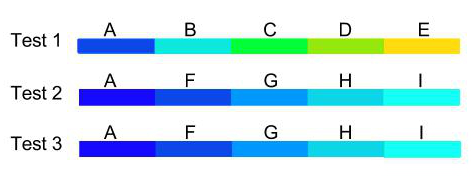
\includegraphics[width=6cm,height=3cm]{spectra.png}
\caption{A spectra where each colour represents different method execution details. We see similarities between Tests 2 and 3. In contrast, Test 1 is different from 2 and 3. }
\label{fig:spectra}
\end{figure}

Once the tests are identified as being redundant, they may be removed, however it is important to understand the dangers of removing test cases. Unless two test cases are exactly the same, it is difficult to guarantee whether one is redundant, even if one subsumes another. This creates the need to be able to use different techniques, dependent on the \DIFdelbegin \DIFdel{project. Therefore to }\DIFdelend \DIFaddbegin \DIFadd{benchmark. To }\DIFaddend expand on the goal of the project, the developed tool should give developers different approaches for identifying redundant test cases. The tool should allow a developer to configure different analysis metrics and view the results. Overall, the tool will be useful for gaining an overview and understanding of the condition of the test suite, allowing for manual inspection to determine if the identified redundant tests should be removed.

Another potential use case of the tool is to redistribute the test cases. This can be achieved by splitting the non redundant tests into another test suite and running this suite in place of the original. The original test suite may be run over night when no development is occurring. This separation of tests based on redundancy allows for a testing process, for example regression testing, to occur in a timely fashion while ensuring the original bug finding ability is retained. This is applicable to David Pearce, \DIFdelbegin \DIFdel{he }\DIFdelend \DIFaddbegin \DIFadd{who }\DIFaddend is currently writing a language called Whiley. The language contains an extended static checking tool to eliminate run time exceptions through formal verification techniques. In the main compiler module alone, there are roughly 20,000 tests. Relocating some these tests into another suite would \DIFdelbegin \DIFdel{result in allowing }\DIFdelend \DIFaddbegin \DIFadd{allow }\DIFaddend him to increase development speed\DIFdelbegin \DIFdel{due to a }\DIFdelend \DIFaddbegin \DIFadd{. This is due to the }\DIFaddend reduction in the time taken to run \DIFdelbegin \DIFdel{a large }\DIFdelend \DIFaddbegin \DIFadd{his }\DIFaddend test suite. \DIFdelbegin \DIFdel{Increasing the frequency of test suite execution also allows for bugs to be traced back }\DIFdelend \DIFaddbegin \DIFadd{This reduction also gives David incentive to execute his suite more often. This increase in frequency allows him to trace back bugs }\DIFaddend to code changes easier and reduces \DIFdelbegin \DIFdel{the }\DIFdelend \DIFaddbegin \DIFadd{his }\DIFaddend time spent debugging. 
\DIFdelbegin \DIFdel{Therefore, by redistributing the test suite, not only does the time taken to run a test suite decrease, there is incentive for developers to execute the suite more often and in turn helping them reduce time taken to debug.
}\DIFdelend 

The contributions of the \DIFdelbegin \DIFdel{report }\DIFdelend \DIFaddbegin \DIFadd{project }\DIFaddend is split into two parts: 

\begin{itemize}
\item Create a tool for identifying redundant test cases
\item Analyse different strategies for identifying redundant test cases through experimenting on realistic benchmarks
\end{itemize}

\section{Outline}

The report is structured as follows. Chapter 2 discusses \DIFaddbegin \DIFadd{previous research in this area of interest. It also examines }\DIFaddend background information and explores the concepts needed to understand the following chapters. \DIFdelbegin \DIFdel{It also examines previous research in this area of interest. }\DIFdelend The design and implementation of the tool is then examined in Chapter 3. Chapter 4 investigates the different techniques \DIFdelbegin \DIFdel{and conducts then }\DIFdelend \DIFaddbegin \DIFadd{then conducts and }\DIFaddend discusses some experiments. Finally, Chapter 5 concludes the report and identifies future work. \newpage 
 \newpage \chapter{Background}\label{C:related}

This chapter \DIFdelbegin \DIFdel{firstly }\DIFdelend explores the current research conducted in this area\DIFdelbegin \DIFdel{, it }\DIFdelend \DIFaddbegin \DIFadd{. It }\DIFaddend then covers the key ideas \DIFdelbegin \DIFdel{that are }\DIFdelend needed to understand the remainder of the report. These ideas are -- approaches to storing method coverage, edit distance metrics, evaluating performance of Java programs and the use of grid computing.

\section{Related Work}
\label{relatedworkRef}
\subsection{Identifying \DIFdelbegin \DIFdel{Redudant }\DIFdelend \DIFaddbegin \DIFadd{Redundant }\DIFaddend Tests}
Testing is a critical part to any software engineering process, not only to stop incidents stemming from the \DIFdelbegin \DIFdel{the }\DIFdelend product, but also partially related to the increase in popularity of agile methodologies \cite{chaos}. Many of these methodologies \DIFdelbegin \DIFdel{employ }\DIFdelend \DIFaddbegin \DIFadd{use }\DIFaddend test driven development and continuous integration\DIFdelbegin \DIFdel{resulting }\DIFdelend \DIFaddbegin \DIFadd{. This results }\DIFaddend in testing becoming more important throughout the development process. For these reasons there have been research papers that examine the different approaches \DIFdelbegin \DIFdel{that can be }\DIFdelend taken to identify redundant test cases and reduce the size of test suites \cite{wong1995effect, wong1999test, rothermel1998empirical, rothermel2002empirical,koochakzadeh2009test,zhang2011empirical,li2008static}.

Whether programmatically reducing a test suite's size is worth the trade off in the ability to locate bugs is unclear.  Wong et al. \cite{wong1995effect, wong1999test} explored the impact that reducing the size of the test suite based off of code coverage had on the fault detection capability. By introducing faults into several programs and comparing the performance between the original and reduced test suites, they found that test suite reduction did not severely impact fault detection capability. In contrast to this finding, Rothermel et al. \cite{rothermel1998empirical, rothermel2002empirical} further expanded on Wong's work by using different benchmark's and performance metrics. They found that test-suite reduction can severely impact the fault detection capability. The \DIFdelbegin \DIFdel{uncertainty created by these conflicting studies }\DIFdelend \DIFaddbegin \DIFadd{conflicting studies create uncertainty. This }\DIFaddend motivates our research to decouple the removal of tests from the \DIFdelbegin \DIFdel{framework }\DIFdelend \DIFaddbegin \DIFadd{tool }\DIFaddend and move the responsibility onto developers. 

A popular technique used in detecting redundancy involves analysing the statement executions, known as statement coverage. Maurer, Garousi and Koochakzadeh \cite{koochakzadeh2009test} attempt to answer the question, \textit{is coverage information enough to determine redundant test cases?} They state a redundant test case as being one that does not improve a specific criteria. For example, Figure \ref{fig:venndiagram} represents the statement criteria data from test cases T1 to T5. The figure shows that T4 and T5 are fully redundant as T3 covers the statements \DIFdelbegin \DIFdel{that are executed by the }\DIFdelend \DIFaddbegin \DIFadd{executed by these }\DIFaddend tests. The authors looked at two other criteria, branch coverage and granularities. Granularity criteria involved splitting the tests into setup, exercise (execution), verify (assert) and lastly teardown then performing analysis over each section. They implemented two different metrics in which both used the criteria described above. The first metric examined each individual test with \DIFdelbegin \DIFdel{respect to }\DIFdelend every other test. It was calculated by measuring the percentage of a test case that is also a subset of \DIFdelbegin \DIFdel{the other }\DIFdelend \DIFaddbegin \DIFadd{another }\DIFaddend test case. The second metric examined each test case with \DIFdelbegin \DIFdel{respect to every }\DIFdelend \DIFaddbegin \DIFadd{the }\DIFaddend test suite as a whole. It was calculated by measuring the percentage of \DIFdelbegin \DIFdel{a }\DIFdelend \DIFaddbegin \DIFadd{the }\DIFaddend test case that \DIFdelbegin \DIFdel{is covered by }\DIFdelend the test suite \DIFaddbegin \DIFadd{covered }\DIFaddend without the test in it. By comparing with manual inspection, they were able to determine the level of false positive and actual redundant tests. Of the redundant tests manually identified, the algorithm matched 95\% of those. However, of the tests that were manually identified as being non-redundant, 52\% of these were identified as being redundant by the algorithm. They concluded that coverage-based information is vulnerable in giving false-positives when identifying redundant test cases, suggesting common code paths as being a root cause. Statement coverage criteria gave a high rate of detection, but the implementation allowed for false positives to impact the results. 

\begin{figure}[h]
\begin{center}
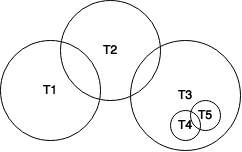
\includegraphics[width=10cm, height=6cm]{VennDiagram.png}
\end{center}
\caption{The coverage of each test is shown by a circle. It shows that T4 and T5 are redundant as T3 already covers those statements.}
\label{fig:venndiagram}
\end{figure}

Zhang, Marinov, Zhang and Khurshid \cite{zhang2011empirical} examined the use of a greedy technique in comparison to heuristics.This required a criteria to be set by the tester, for example, statement coverage. The greedy technique would greedily select a test case that satisfies the maximum number of unsatisfied test requirements\DIFdelbegin \DIFdel{and }\DIFdelend \DIFaddbegin \DIFadd{. It }\DIFaddend would continue until all the test requirements had been satisfied. \DIFdelbegin \DIFdel{So the }\DIFdelend \DIFaddbegin \DIFadd{The }\DIFaddend new test suite will contain exactly the same coverage as the old test suite while removing redundant test cases. This means that if a test subsumed another, then it would always be removed. The heuristic implementation was first conceived by Harrold, Gupta and Soffa \cite{harrold1993methodology} where \DIFaddbegin \DIFadd{it selects }\DIFaddend essential test cases \DIFdelbegin \DIFdel{are selected }\DIFdelend as early as possible. Essential being that only one test case satisfies a test requirement exclusively. The heuristic approach resulted in the most cost-effective reduction, this being the amount of reduction and the fault-detection capability of the reduced test suites\DIFdelbegin \DIFdel{, showing }\DIFdelend \DIFaddbegin \DIFadd{. This showed }\DIFaddend that although greedy approach worked, there were better techniques available.

In situations where it is not possible to generate a spectrum to analyse, static analysis can be used to determine the level of redundancy. Robinson, Li and Francis \cite{li2008static} \DIFdelbegin \DIFdel{examine }\DIFdelend \DIFaddbegin \DIFadd{explore }\DIFaddend this. The tests for the benchmark they use are written in a high level automation framework and consist of a list of commands. The commands perform actions such as file copying and loading configurations. To identify redundant test cases they examine the test case commands as well as the instructions within the procedures that the test case loads. To calculate the similarities between two test cases, they consider three different metrics\DIFdelbegin \DIFdel{, }\DIFdelend \DIFaddbegin \DIFadd{. These are the }\DIFaddend Manhattan distance, unigram cosine similarity and bigram cosine similarity. They each were measuring how closely related two tests were based on the sequence of commands and procedures loaded. Their findings were similar to Maurer et al. \cite{koochakzadeh2009test} in that there are a large number of false positives. Static checking has several limitations in comparison to dynamic. The main disadvantage is the availability of data. During run-time is when a large portion of the data trail is available\DIFdelbegin \DIFdel{and }\DIFdelend \DIFaddbegin \DIFadd{. This }\DIFaddend is important when needing to know the exact method calls and parameters passed to these methods. Static checking would provide useful information in a framework where dynamic data can not be collected. The framework would also need to be applicable to being examined in a static fashion such as the one used by Robinson, Li and Francis \cite{li2008static}.

Taking into the related work discussed, each paper used the coverage of a test suite at several different criterion levels but none looked at the method execution explicitly. This leaves a potentially useful approach to the problem that may help determine the level of redundancy within a test suite. 
\subsection{Calling Tree}
When methods execute there is a trail of data that is left behind. Piecing together this data can show the relationships between methods, which is known as a \textit{call graph}. The call graph can be retrieved statically or dynamically \cite{graham1982gprof}. A static graph represents every possible run of the program. A dynamic graph represents one particular run. Comparing them, a static graph requires more information to be held\DIFdelbegin \DIFdel{and in }\DIFdelend \DIFaddbegin \DIFadd{. In }\DIFaddend the particular case of profiling test cases, dynamic would be more suitable due to the nature of a test case being the same for every run. Another advantage of a dynamic graph is the ability to collect functional parameters. Xiaotong Zhuang and et al. \cite{Zhuang06accurate} describe a call tree as the overall tree of every method execution. To store the full call tree would involve an excess of memory, therefore they discuss the use of a calling context tree. This tree represents the same method executions however is compressed where the edge between the nodes contains a weighting, the weighting being the number of occurrences of that method execution (calling frequency). Examining Figure \ref{fig:callgraph} shows the different variations that can be observed with the same data. The top left hand picture shows the method execution trail, where A calls B, then B calls D twice and A calls C, then C calls D once. The call graph image (top right) condenses the information into one node per method call. This method is the most condensed variation, but gives the least amount of information. Directly below this, the calling context tree condenses it slightly less. It separates each path into its own branch when it is unique to the tree\DIFdelbegin \DIFdel{, the }\DIFdelend \DIFaddbegin \DIFadd{. The }\DIFaddend connection between nodes contains a weighting which \DIFdelbegin \DIFdel{represent }\DIFdelend \DIFaddbegin \DIFadd{represents }\DIFaddend the frequency. Finally, the bottom left (call tree) creates a new path for every new method execution regardless of the uniqueness\DIFdelbegin \DIFdel{, giving us the }\DIFdelend \DIFaddbegin \DIFadd{. This allows for the tree to retain the }\DIFaddend most information about the context\DIFdelbegin \DIFdel{if the order is retained}\DIFdelend .

\begin{figure}[h]
\begin{center}
\includegraphics[width = \textwidth]{CallGraph.png}
\end{center}
\caption{A diagram showing the three different variations of Call Graph information. Where  each have a varying level of information that is stored.}
\label{fig:callgraph}
\end{figure}

\subsection{Edit Distance Metrics}
\label{editdistbg}
Edit distance algorithms play an important part in many domains, ranging from signal processing to mutations in genome sequences \cite{navarro2001guided}. They calculate the number of edit operations needed to go from one string to another, in our research they are used to calculate the difference between test \DIFdelbegin \DIFdel{case spectras}\DIFdelend \DIFaddbegin \DIFadd{spectrums}\DIFaddend . There are a variety of different implementations of edit distance metrics. Cohen, Ravikumar and Fienberg \cite{cohen2003comparison} explore different edit distance metrics for name matching. They concluded that Monge and Elkan \cite{monge1997efficient} performed the best for string edit-distance metrics. The metric works by splitting the two strings into tokens, the best matching tokens are then calculated to find the similarity using other common metrics such as Levenshtein distance. One of the other techniques they explored was the Levenshtein distance \cite{levenshtein1966binary} metric by itself. This metric is the minimal number of operations \DIFdelbegin \DIFdel{that can be done to make }\DIFdelend \DIFaddbegin \DIFadd{to change }\DIFaddend one test's spectrum \DIFdelbegin \DIFdel{equal to }\DIFdelend \DIFaddbegin \DIFadd{into }\DIFaddend another. These operations are inserting, deleting or substituting and a cost is associated with completing an operation. The maximum difference is the size of the larger spectra. The amount of redundancy is calculated by dividing the cost of operations with the max difference in order to normalize the value. This value is the percentage of the test that is not redundant, the value 1 is then subtracted by the value to give the redundant percentage.

\DIFdelbegin \DIFdel{An }\DIFdelend \DIFaddbegin \DIFadd{Table \ref{levenTable} shows an }\DIFaddend example of Levenshtein\DIFdelbegin \DIFdel{is shown in Table \ref{levenTable}, where }\DIFdelend \DIFaddbegin \DIFadd{. The example changes }\DIFaddend 'kitchen' \DIFdelbegin \DIFdel{is being changed }\DIFdelend into 'kitten'. \DIFdelbegin \DIFdel{The example }\DIFdelend \DIFaddbegin \DIFadd{It }\DIFaddend shows the number of operations needed is 2, and the max potential needed if the two strings were completely different is 7, as kitchen contains 7 characters. The redundancy is calculated by subtracting 1 from the cost over the max potential cost $(1 - (2/7)) $. The outcome being that the words contain 71\% redundant information. 

\begin{table}[H]
\centering

\begin{tabular}{|l|l|l|}
\hline
{\bf Previous State} & {\bf Current State} & {\bf Operation}                      \\ \hline
-                    & kitten              & -                                    \\ \hline
kitten               & kitcen              & Substitution of `t' with `c'         \\ \hline
kitcen               & kitchen             & Insertion of `h' between `c' and `e' \\ \hline
\end{tabular}
\caption{Using Levenshtein edit distance metric to transform kitten to kitchen.}
\label{levenTable}
\end{table}

\DIFdelbegin \DIFdel{An }\DIFdelend \DIFaddbegin \DIFadd{Table \ref{mongeTable} shows an }\DIFaddend example of Monge \& Elkan\DIFdelbegin \DIFdel{is shown in Table \ref{mongeTable}. The comparison of }\DIFdelend \DIFaddbegin \DIFadd{. It compares }\DIFaddend the strings `paul johnson' and `johson paule'\DIFdelbegin \DIFdel{are being compared}\DIFdelend . Each of the strings get broken down into two tokens and the best matches are identified and used for the final score. The table shows that the final score of the Monge \& Elkan is taking into account `paul' \& `paule' and `johnson' \& `johson'. Using these two matches, the final result is 1/2 * (.85 + .80) = 0.825.

\begin{table}[H]
\centering

\begin{tabular}{|l|l|}
\hline
\textbf{Input string 1:}        & paul johnson \\ \hline
\textbf{Input string 2:}        & johson paule \\ \hline
                                &              \\ \hline
Levenshtein("paul","johson")    & 0.00         \\ \hline
Levenshtein("paul","paule")     & 0.80         \\ \hline
Levenshtein("johnson","paule")  & 0.00         \\ \hline
Levenshtein("johnson","johson") & 0.85         \\ \hline
\end{tabular}
\caption{The Monge \& Elkan edit distance metric to calculate the similarity between "paul johnson" and "johson paule"}
\label{mongeTable}
\end{table}



\subsection{Wilcoxon Signed Rank Test}

A Wilcoxon Signed Rank test is used to infer whether there are any significant differences between the techniques implemented in this report. The Wilcoxon Signed Rank test was first proposed by Frank Wilcoxon in 1945 \cite{wilcoxon1945individual}. It is a nonparametric test for comparing two pair groups. A nonparametric test is a collective term that is given to inferences that are valid under less confining assumptions than classical statistical inferences \cite{nonparametric}. The test does not assume that the data follows a normal distribution which is ideal for the data presented in our research and is used when two nominal variables and one measure variable is being measured \cite{mcdonald2009handbook}.

\section{Performance Evaluation}
\label{performanceEvalBG}
Throughout the report different techniques are designed and implemented to identify redundant test cases. To evaluate the techniques, experiments are conducted and must adhere to a standard procedure. The purpose for evaluating the performance of a given technique is to create an understanding of the typical performance. For this typical performance to be valid, it has to be rigorous in design and implementation. This involves taking into consideration a variety of factors that will be examined in reference to research papers that explore the issues.

Andy Georges et al. \cite{georges2007statistically} and Steve Blackburn et al. \cite{blackburn2008wake} present issues and alternatives to the current Java performance methodologies used in research papers. They note that in premier conferences, 16 of the 50 papers examined did not discuss the methodology they used. This limits the validity of the results and creates a situation where the experiment cannot be reproduced. One of the main issues identified is specifying singular numbers, without expressing what the number is referring to (average, median, best, worst). This leads to a misleading representation of the results. A set of parameters that are of interest are explored in the paper, these include, heap size, start up performance, number of virtual machine (VM) invocations and handling of garbage collection. An experiment should also take into consideration the environment that the analysis is executed on:
\begin{itemize}
\item \textbf{Heap Size} -- A change in heap size can impact the garbage collection process. The smaller the heap size, the more often the garbage collector is run.
\item \textbf{Start Up Costs}  -- The costs associated with starting the application up. This will always involve class loading and just in time (JIT) re(compilation), it can also involve reading from a database and setting the application up.
\item \textbf{Number of VM invocations} -- The number of application runs that a single VM instance will execute.
\item \textbf{Garbage Collection} -- The process in identifying and removing objects that are no longer referenced.
\item \textbf{Environment} -- The hardware that the application is being run on.
\end{itemize}

\section{Grid Computing}
The time intensive nature of conducting the experiments resulted in a single computer not being adequate. A grid computing system was used instead, it is a distributed system of multiple machines that have no interactive tasks between each other. No interactions results in task independence being a necessity. The particular grid system used for this report is located at Victoria University of Wellington. The machines in the grid are idle machines around the School of Engineering and Computer Science. There are a limited number of machines, therefore a total of 150 jobs can be run at a given time. Since the grid is located around an active community, if a user logs on while a process is being conducted, the application is paused until the machine returns to an idle state. \newpage 
 \newpage \chapter{Design and Implementation}\label{C:workdone}

\section{Overview}

The goal of the project as mentioned in Section \ref{C:intro} is to create a tool to allow developers to identify redundant test cases. The tool \DIFdelbegin \DIFdel{can be }\DIFdelend \DIFaddbegin \DIFadd{is }\DIFaddend split into several different sections and \DIFdelbegin \DIFdel{each section will be discussed in this chapter }\DIFdelend \DIFaddbegin \DIFadd{the chapter will discuss each}\DIFaddend . The first objective of the tool was to trace the test data. We \DIFdelbegin \DIFdel{explored }\DIFdelend \DIFaddbegin \DIFadd{explore }\DIFaddend two different frameworks and \DIFdelbegin \DIFdel{compared }\DIFdelend \DIFaddbegin \DIFadd{compare }\DIFaddend the usability of each. After the tool was able to trace the data, we \DIFdelbegin \DIFdel{had to }\DIFdelend determine what spectras we \DIFdelbegin \DIFdel{were }\DIFdelend \DIFaddbegin \DIFadd{are }\DIFaddend interested in. \DIFdelbegin \DIFdel{The three different spectra types }\DIFdelend \DIFaddbegin \DIFadd{These }\DIFaddend are then discussed. The \DIFdelbegin \DIFdel{data traced from each test case was then compared to that from every other test to determine the level of redundancy. The comparison was done with }\DIFdelend \DIFaddbegin \DIFadd{next section then discusses using }\DIFaddend edit distance metrics \DIFaddbegin \DIFadd{to compare test case trace information}\DIFaddend . Throughout the testing of the tool, one of the main impediments was the time taken to analyse the large amount of data. We examine how breaking the analysis into a series of pipeline stages decreases the time taken.

\section{Tracing}
\label{S:trace}
A fundamental requirement for this project was to trace \DIFdelbegin \DIFdel{which methods were }\DIFdelend \DIFaddbegin \DIFadd{the methods }\DIFaddend executed by a test. David Pearce's language Whiley is written in Java\DIFaddbegin \DIFadd{, }\DIFaddend therefore it was decided to use Java frameworks to trace the tests. There were two tracing \DIFdelbegin \DIFdel{frameworks }\DIFdelend \DIFaddbegin \DIFadd{framework's }\DIFaddend considered. The first framework considered was AspectJ. The technique that AspectJ uses is \DIFdelbegin \DIFdel{called }\DIFdelend Aspect Oriented Programming (AOP). AOP can be used to add code to an existing program without modifying the source code\DIFdelbegin \DIFdel{, this code added is known as }\DIFdelend \DIFaddbegin \DIFadd{. AspectJ uses }\DIFaddend an \textit{aspect} \DIFdelbegin \DIFdel{. This process }\DIFdelend \DIFaddbegin \DIFadd{to identify where and what is added. This can }\DIFaddend be achieved through the following methods:

\begin{itemize}
\item \textbf{Compile time} --
The classes are compiled with the aspect woven into them. When the program is executed, the methods have the code from the aspect woven into \DIFdelbegin \DIFdel{it }\DIFdelend \DIFaddbegin \DIFadd{them }\DIFaddend already. This requires the source to be compiled with AspectJ's compiler.
\item \textbf{Load time} --
The weaving process is deferred until the point at which a class loader attempts to load in a class file. Load time modification is achieved by using a command line argument notifying Java to use the AspectJ class loader.
\end{itemize}

The other framework we considered was the Java Debugging Interface (JDI). JDI is similar to using an observer pattern. \DIFdelbegin \DIFdel{A }\DIFdelend \DIFaddbegin \DIFadd{It selects a }\DIFaddend list of classes to observe \DIFdelbegin \DIFdel{are selected. When }\DIFdelend \DIFaddbegin \DIFadd{and when }\DIFaddend a method within a selected class is called, the listener class is notified\DIFdelbegin \DIFdel{and is given }\DIFdelend \DIFaddbegin \DIFadd{. This class is then passed }\DIFaddend the information about the method call. 

AspectJ provided several advantages over JDI. The ability to choose which methods to record was easier to define and it returns the actual object when retrieving the parameters of the method call. This detail becomes important when we explore tracing parameter values in Section \ref{parameterTrace}. In comparison, JDI was faster to execute, however there was a limited amount of documentation available and the parameters returned were not the actual objects. The decision to use AspectJ was based off this trade off between information and performance. Decoupling the data gathering and data analysis within the tool removed the emphasis on retrieval performance\DIFdelbegin \DIFdel{and resulted in the extra information being more important}\DIFdelend \DIFaddbegin \DIFadd{. This meant that the tracing performance was less of an issue}\DIFaddend .

To distinguish what code to weave, and where in the existing code to weave it, AspectJ uses a \textit{\DIFdelbegin \DIFdel{point cut}\DIFdelend \DIFaddbegin \DIFadd{pointcut}\DIFaddend } \cite{aspectj}. \DIFdelbegin \DIFdel{A point cut was made to record every execution}\DIFdelend \DIFaddbegin \DIFadd{Our pointcuts record every method execution. Figure \ref{fig:aspectused} shows a simplified version}\DIFaddend . \DIFdelbegin \DIFdel{A simplified version of the aspect is shown in Figure \ref{fig:aspectused} . }\DIFdelend There are two \DIFdelbegin \DIFdel{point cuts }\DIFdelend \DIFaddbegin \DIFadd{pointcuts }\DIFaddend within the aspect\DIFdelbegin \DIFdel{, the first point cut is going to be }\DIFdelend \DIFaddbegin \DIFadd{. The first pointcut gets }\DIFaddend called for every method call which has a \DIFdelbegin \DIFdel{junit }\DIFdelend \DIFaddbegin \DIFadd{JUnit }\DIFaddend \@Test annotation attached to it. This will then call a static service passing it the method information of the new test. The second \DIFdelbegin \DIFdel{point cut is used to trace }\DIFdelend \DIFaddbegin \DIFadd{pointcut traces }\DIFaddend everything apart from \DIFaddbegin \DIFadd{the }\DIFaddend methods with a \DIFaddbegin \DIFadd{JUnit }\DIFaddend \@Test annotation attached\DIFdelbegin \DIFdel{and passed }\DIFdelend \DIFaddbegin \DIFadd{. It then passes }\DIFaddend the information to the static service. The next stage was to weave the aspect into \DIFdelbegin \DIFdel{the }\DIFdelend \DIFaddbegin \DIFadd{a }\DIFaddend benchmark. Using compile time weaving would have meant that \DIFdelbegin \DIFdel{each benchmark needed }\DIFdelend \DIFaddbegin \DIFadd{every benchmark had }\DIFaddend to be recompiled using the aspect compiler. In contrast, load time only requires the AspectJ class loader to be passed through a command line argument. Load time was chosen as it was easy to use when working with external benchmarks.

\begin{figure}[h]
\begin{center}
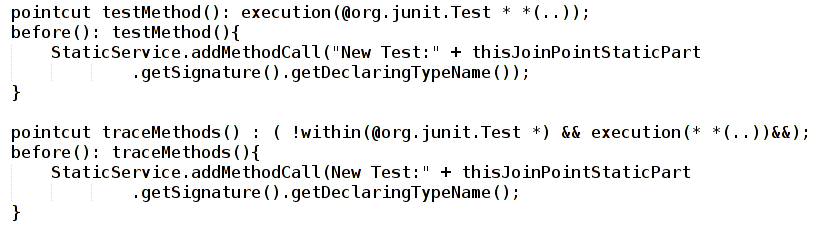
\includegraphics[width = \textwidth]{aspect.png}
\end{center}
\caption{A simplified \DIFdelbeginFL \DIFdelFL{point cut }\DIFdelendFL \DIFaddbeginFL \DIFaddFL{pointcut }\DIFaddendFL within AspectJ. The first \DIFdelbeginFL \DIFdelFL{point cut }\DIFdelendFL \DIFaddbeginFL \DIFaddFL{pointcut }\DIFaddendFL is for when a new test is executed and the second when a new method is executed.}
\label{fig:aspectused}
\end{figure}

\DIFaddbegin \subsection{\DIFadd{Saving to the Network}}
\DIFadd{To execute the analysis on a grid computing system, the test data had to accessible on the School of Engineering's local network. To achieve this, the trace data was saved to the local network. Not only did it allow for the analysis to be executed on the grid system, it also it allowed for the data to be reanalysed without having to re trace the test suite. 
}

\DIFaddend \section{Filtering By Spectra \DIFdelbegin %DIFDELCMD < \improvement{Dave}%%%
\DIFdelend }
\label{S:spectra}
The idea of a spectrum was previously identified in Chapter \ref{C:intro}. Reexamining the idea, a spectrum is some abstraction of the method information. There are three different types of spectrum\DIFdelbegin \DIFdel{, these }\DIFdelend \DIFaddbegin \DIFadd{. These }\DIFaddend are \textit{unique method calls}, \textit{all method calls} and \textit{call tree}, each with its own characteristic. It is important to understand how we use a spectra. When the tool is tracing the tests, it traces the amount of information needed based on a settings file. A spectra can then \DIFaddbegin \DIFadd{be }\DIFaddend applied to this trace information to filter out data to match the spectras characteristic. The tool ensures that the traced information is able to be filtered by the spectra. 

We will examine the spectra characteristics in relation to the example shown in Figure \ref{fig:callingexample}. The different spectra's take up different levels of resources, these are are\DIFdelbegin \DIFdel{-- }\DIFdelend \DIFaddbegin \DIFadd{: }\DIFaddend time taken and memory. 


\begin{figure}[h]
\begin{center}
\DIFdelbeginFL %DIFDELCMD < \includegraphics[height = 4cm]{callingexample.png}
%DIFDELCMD < %%%
\DIFdelendFL \DIFaddbeginFL \includegraphics[height = 6cm]{callingexample.png}
\DIFaddendFL \end{center}
\caption{A simple representation of a call tree of three that is traced from a test. Each letter represents a method call and the bold letter is the active method in each line of the call tree.}
\label{fig:callingexample}
\end{figure}

\subsection{Unique Method Calls}
The "unique method call" spectra filters out the repetition of methods. The data \DIFdelbegin \DIFdel{from }\DIFdelend \DIFaddbegin \DIFadd{after }\DIFaddend applying the filter only has each method represented a single time. The motivation of this spectra is to substantially reduce the time taken and memory used. Consequently, decreasing the amount of data leads to a decrease in the confidence that the tests identified are truly redundant. 

Examining Figure \ref{fig:callingexample}, \DIFdelbegin \DIFdel{the method calls are }\DIFdelend \DIFaddbegin \DIFadd{on the left hand side are the method calls where each line represents one call. The active method is in bold and the parent methods are before it. On the right hand side is the call tree. With no filtering applied the method calls are }\DIFaddend "\DIFaddbegin \DIFadd{A,}\DIFaddend B,C,D,C,B,D". When we \DIFdelbegin \DIFdel{use a unique method call spectra to filterthis trace information}\DIFdelend \DIFaddbegin \DIFadd{apply a "unique method calls" spectrum filter}\DIFaddend , the data will become "\DIFaddbegin \DIFadd{A,}\DIFaddend B,C,D". This shows that we are filtering out a large portion of data while retaining an adequate representation of the original trace information. We can explore how this effects the Whiley Compiler benchmark. There are 494 unique methods called for a particular test and 80,000 method executions. Utilising the unique method call spectra, the tool will only use 494 method executions when comparing the test with another, rather than the 80,\DIFdelbegin \DIFdel{000, }\DIFdelend \DIFaddbegin \DIFadd{000. This is }\DIFaddend $\rfrac{6}{1000}$ of the original amount. 

\subsection{All Method Calls}
The "all method calls" \DIFdelbegin \DIFdel{spectra }\DIFdelend \DIFaddbegin \DIFadd{spectrum }\DIFaddend filters out information regarding the call tree. The motivation behind this approach is to \DIFdelbegin \DIFdel{increase our confidence with the results , but }\DIFdelend \DIFaddbegin \DIFadd{analyse a larger subset of trace data than the "unique method calls" spectra. Comparing the two, "all method calls" increases our confidence in the results however, }\DIFaddend this increases the time taken and memory used to analyse the information.

Examining Figure \ref{fig:callingexample}, the output of filtering \DIFaddbegin \DIFadd{the method calls }\DIFaddend with this spectra would be "\DIFaddbegin \DIFadd{A,}\DIFaddend B,C,D,C,B,D". This shows a loss of the context data. We can explore how this effects the Whiley Compiler benchmark. When using an "all method calls" spectra, the tool will use all 80,000 method executions when comparing the test with another.

\subsection{Call Tree}
A "call tree" may filter out some of the parent methods. The number of calls retained is referred to as the K depth \cite{Zhuang06accurate}. The motivation behind the approach is to increase our confidence in the results by taking into account the \textit{context} of a call. The consequence of increasing the amount of data is \DIFdelbegin \DIFdel{an }\DIFdelend \DIFaddbegin \DIFadd{a further }\DIFaddend increase in the time taken and memory used to analyse the trace data \DIFdelbegin \DIFdel{but a further increase in the confidence in }\DIFdelend \DIFaddbegin \DIFadd{in }\DIFaddend comparison to the other two \DIFdelbegin \DIFdel{spectras}\DIFdelend \DIFaddbegin \DIFadd{spectrums}\DIFaddend .

We can filter the Figure \ref{fig:callingexample} using a K depth of two. This would lead to the filtered data returning 'A\DIFaddbegin \DIFadd{, A }\DIFaddend $\rightarrow$ B', 'B $\rightarrow$ C', 'A $\rightarrow$ D', 'D $\rightarrow$ C', 'A $\rightarrow$ B' and 'B $\rightarrow$ D'. We can see that by using a K depth of two, we lose some of the information from the trace data. To stop this loss of data, we could extend the depth to three. Using the Whiley Compiler benchmark as an example, a \DIFdelbegin \DIFdel{calling context spectra }\DIFdelend \DIFaddbegin \DIFadd{call tree filter with a depth of 3 }\DIFaddend would examine all \DIFdelbegin \DIFdel{80}\DIFdelend \DIFaddbegin \DIFadd{240}\DIFaddend ,000 method executions\DIFdelbegin \DIFdel{, with each containing K depth of method calls. }\DIFdelend \DIFaddbegin \DIFadd{. The extra data occurs from storing each of the method executions two parent methods. As we use a call tree representation, the duplicated nodes are repeated in the tree. 
}\DIFaddend 

To retrieve the calling context in Java, the current stack trace of a method call is examined\DIFdelbegin \DIFdel{and }\DIFdelend \DIFaddbegin \DIFadd{. It is }\DIFaddend then parsed to retrieve the relevant information. This parsing involves removing the method calls that are used to retrieve the stack trace and any memory location details. 

\section{Analysis Metrics\DIFdelbegin %DIFDELCMD < \improvement{Dave}%%%
\DIFdelend }
\label{S:metrics}
\DIFdelbegin \DIFdel{The data traced }\DIFdelend \DIFaddbegin \DIFadd{Having traced the information and being able to filter out specific data. This filtered data then }\DIFaddend needs to be \DIFdelbegin \DIFdel{analysed }\DIFdelend \DIFaddbegin \DIFadd{then compared with another test cases data }\DIFaddend to produce a \DIFdelbegin \DIFdel{quantitative value. The value produced will be used to determine the level of similarity between two test cases}\DIFdelend \DIFaddbegin \DIFadd{redundant level between them}\DIFaddend . Edit distance metrics were \DIFaddbegin \DIFadd{choosen to perform this comparison. They were }\DIFaddend discussed in Section \ref{editdistbg}, with two different edit distance metrics considered. They were: Monge \& Elkan \cite{monge1997efficient} which splits the strings into sections and compares the sections and Levenshtein \cite{levenshtein1966binary} which compares tokens that are generally single characters. 

For both of the algorithms, there were publicly available frameworks that implemented them. Both implementations allowed for a call tree to be represented by a token. The \DIFdelbegin \DIFdel{test cases trace information was repreesnted }\DIFdelend \DIFaddbegin \DIFadd{trace information of the test cases were represented }\DIFaddend by a list of tokens. The issue with Monge \& Elkan was it attempted to find the best match with no regard to the ordering. Attempting to find the best match would increase the time taken, perform unnecessary computation for our requirements and increase the false positive rate. The trace information in Figure \ref{fig:mongevleven} can be used to show the difference between \DIFaddbegin \DIFadd{the }\DIFaddend metrics. The implementation of Monge \& Elkan would match 'Method Call' in test case 1 to the 'Method Call' in test case 2, even though they were called at different times. Levenshtein did not search for a match, rather the metric only looked at the opposing method call. This direct matching was preferred as we were interested in the order of the method calls as well as what methods were called.

\begin{figure}[h]
\begin{center}
\includegraphics[width = \textwidth]{MongeVLeven.png}
\end{center}
\caption{Trace information used to show the difference between Monge \& Elkan and Levenshtein metric implementations. The Monge \& Elkan metric will disregard ordering and measure these test cases as being the same. The Levenshtein metric examines one to one and will measure the test cases as having no similarities.}
\label{fig:mongevleven}
\end{figure}

\section{Pipeline \DIFdelbegin %DIFDELCMD < \improvement{Dave}%%%
\DIFdelend }
\label{pipelinesection}
For the tool to help developers reduce the number of redundant tests, it has to analyse the information within an acceptable time frame. Comparing every test with every other while using all \DIFdelbegin \DIFdel{of }\DIFdelend the available information (\DIFaddbegin \DIFadd{e.g. }\DIFaddend call tree) in some cases resulted in the analysis taking several days to complete. This is not considered an acceptable time frame. This issue arises when each of the spectrum of the test cases contain tens of thousands of method calls. \DIFdelbegin \DIFdel{To get around the }\DIFdelend \DIFaddbegin \DIFadd{A pipeline approach was implemented to get around this }\DIFaddend issue of lengthy analysis\DIFdelbegin \DIFdel{, a pipeline approach was implemented. The idea is visualized in Figure \ref{fig:pipeline} }\DIFdelend . \DIFaddbegin \DIFadd{Figure \ref{fig:pipeline} visualises the idea. }\DIFaddend The figure shows the trace information is input into the start of the pipeline. The purpose of a stage is to determine the redundancy of test pairs. If a pair is \DIFdelbegin \DIFdel{within }\DIFdelend \DIFaddbegin \DIFadd{larger }\DIFaddend the redundancy limit specified, it will \DIFdelbegin \DIFdel{then be kept }\DIFdelend \DIFaddbegin \DIFadd{be stored }\DIFaddend and analysed during the next stage. The goal is that each subsequent stage should soundly eliminate pairs from consideration that the following stages would have removed. \DIFdelbegin \DIFdel{This goal can be achieved by using heuristics}\DIFdelend \DIFaddbegin \DIFadd{Heuristics can help achieve this goal}\DIFaddend . A heuristic would examine a subset of data while still eliminating test pairs that would have been removed in the subsequent stages. 

\begin{figure}[h]
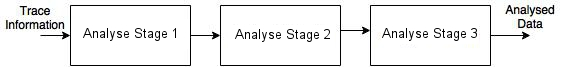
\includegraphics[width=\textwidth]{Pipeline.jpg}
\caption{Trace information goes in at the start of the pipeline. After each stage there should be a reduction of comparisons that the next stage has to complete. The last stage should be the most computationally heavy.}
\label{fig:pipeline}
\end{figure}

To further expand on the heuristic idea\DIFdelbegin \DIFdel{. By utilising different spectra filters , this allows for }\DIFdelend \DIFaddbegin \DIFadd{, the tool can use the spectra filters to examine }\DIFaddend the trace information \DIFdelbegin \DIFdel{to be examined with different characteristics}\DIFdelend \DIFaddbegin \DIFadd{in different perspectives}\DIFaddend . The particular filter of interest is the "unique method calls" spectra. Inspecting a subset of the trace data increased the speed of the comparison but as a consequence, it decreased the confidence of the output being truly redundant. We can increase the confidence by then analysing the output test pairs with a "context tree" filter. An important part to emphasize is that no information is lost when information is filtered, rather some of it is ignored for that pipeline \DIFaddbegin \DIFadd{stage }\DIFaddend only. We see a pipeline set up in Figure \ref{fig:pipelineExample}. The first stage uses a "unique method calls" spectra and pipelines the output into a "call tree" of depth thee. The three test cases at the top are the trace information input into the pipeline. The remainder of this section explores this example. 

\paragraph{Pipeline Stage 1}
The tool first filters the trace information with a "unique method call" spectra. The three test cases are filtered into:

\begin{enumerate}
\item "B,C,D" 
\item "E,H,J,M,Q"
\item "B,C,D"
\end{enumerate}

Calculating the Levenshtein distance between each, it would show that test cases 1 and 3 are similar but test case 2 has no similarities to either. The test cases that are passed onto the next pipeline stage are test cases 1 and 3.

\paragraph{Pipeline Stage 2}

The information used in this stage is shown at the top of the figure. The only test cases \DIFdelbegin \DIFdel{examined }\DIFdelend \DIFaddbegin \DIFadd{compared }\DIFaddend are test cases 1 and 3. Looking at the test cases, when filtered with a call tree of depth three there are no similarities between the two method calls. \DIFdelbegin \DIFdel{The }\DIFdelend \DIFaddbegin \DIFadd{This is because that highest level calls are different between them. Hence the }\DIFaddend output of the pipeline as a whole is \DIFaddbegin \DIFadd{that }\DIFaddend there are no redundant test cases in the trace information.

\begin{figure}[h]
\includegraphics[width=\textwidth]{callingexampleExtra.png}
\caption{A two stage pipeline that analyses the trace information shown. The first stage uses a "unique method calls" filter with a 98\% similarity and the second stage filters with a call tree of K Depth three with a 98\% similarity. After analysing the data, no test cases are returned as being redundant.}
\label{fig:pipelineExample}
\end{figure}

\DIFdelbegin \DIFdel{This example contains a pipeline of length two. When using a pipeline of length three, }\DIFdelend \DIFaddbegin \DIFadd{An alternative heuristic to use is }\DIFaddend the "all method calls" spectra\DIFdelbegin \DIFdel{may be used as the second stage heuristic. The "all method calls" spectra would not be appropriate in the last pipeline as there is limited sense in using a subset of data.
}%DIFDELCMD < 

%DIFDELCMD < %%%
\DIFdel{The list spectra may also be used as another type of heuristic. The motivation behind the spectra is to be used as the second stage in a three stage pipeline. }\DIFdelend \DIFaddbegin \DIFadd{. }\DIFaddend In comparison to the "unique method calls" filter, the "all method calls" \DIFdelbegin \DIFdel{increases }\DIFdelend \DIFaddbegin \DIFadd{filter further decreases }\DIFaddend the amount of comparisons that the final pipeline \DIFdelbegin \DIFdel{should and with more }\DIFdelend \DIFaddbegin \DIFadd{does. It then leads to an increase in }\DIFaddend confidence of the results \DIFdelbegin \DIFdel{however, increases time taken }\DIFdelend \DIFaddbegin \DIFadd{but also, an increase in the time taken and memory consumption}\DIFaddend . This approach \DIFdelbegin \DIFdel{would not be used in the last pipeline as there is limited sense to use a subset of information retrieved from the test cases. }\DIFdelend \DIFaddbegin \DIFadd{may be used as the last stage in a pipeline of the length two. The other option, would be to have it as the middle stage in a pipeline of length three.
}\DIFaddend 

\DIFdelbegin \subsection{\DIFdel{Saving to the Network}}
%DIFAUXCMD
\addtocounter{subsection}{-1}%DIFAUXCMD
\DIFdel{To execute the analysis on a grid computing system, the test data had to accessible on the School of Engineering's local network.
To achieve this, the trace data was saved to the local network. Not only did it allow for the analysis to be executed on the grid system, it also it allowed for the data to be reanalysed without having to re execute the test suite. 
}%DIFDELCMD < 

%DIFDELCMD < %%%
\DIFdelend \section{Tracing Parameter Values}
\label{parameterTrace}
The related work in this research area has explored using statement coverage while ignoring the parameter values of each method. It could be argued that due to knowing the statement path, parameters are irrelevant as you know the path the method will take, and parameters do not add any more information. When tracing at the method level rather than at the statement level, parameters become crucial to determine the degree of redundancy between test cases. This is because parameters give insight into the execution paths that will be taken and act as a proxy to the statement information without storing the same amount of the data.

There were two variations of parameters that were considered to trace. Firstly, primitive types only. \DIFdelbegin \DIFdel{By }\DIFdelend \DIFaddbegin \DIFadd{Primitives only represented a small number of parameters when }\DIFaddend running test experiments on the benchmarks\DIFdelbegin \DIFdel{, the use of primitives showed that only a limited number of parameters were collected}\DIFdelend .  The parameters collected had a limited effect on the number of false positives identified and time taken. The second approach \DIFdelbegin \DIFdel{is }\DIFdelend \DIFaddbegin \DIFadd{was }\DIFaddend to use reflection. Reflection is the ability to examine and modify objects at run time \cite{oraclereflection}. Since AspectJ gives direct access to the object's within the method parameters, reflection can be used. By using reflection, \DIFaddbegin \DIFadd{we retrieve }\DIFaddend the fields of the \DIFdelbegin \DIFdel{objects are retrieved and returned }\DIFdelend \DIFaddbegin \DIFadd{object and return them }\DIFaddend in a string to represent the state of the object. If there are objects within the object, a reference is returned to ensure no cycles occur. This string is then examined to remove any Java reference locations and then stored. The reflection is done through \DIFdelbegin \DIFdel{Apaches }\DIFdelend \DIFaddbegin \DIFadd{the Apache }\DIFaddend commons language library. \DIFaddbegin \DIFadd{We decided to use reflection as it represented a method call more than primitive types.
}\DIFaddend 

The most common use case of the tool is expected to use parameters\DIFdelbegin \DIFdel{therefore it was }\DIFdelend \DIFaddbegin \DIFadd{. It was therefore }\DIFaddend decided to optimize this through storing the data with \DIFdelbegin \DIFdel{parameters}\DIFdelend \DIFaddbegin \DIFadd{them}\DIFaddend . The optimization involved saving the parameters \DIFdelbegin \DIFdel{with the trace information}\DIFdelend \DIFaddbegin \DIFadd{directly onto the method executions}\DIFaddend . If parameters \DIFdelbegin \DIFdel{value is set to false, the parameters }\DIFdelend \DIFaddbegin \DIFadd{were not required, they }\DIFaddend have to be split off rather than being concatenated on. This \DIFdelbegin \DIFdel{means that setting the parameters to false would increase }\DIFdelend \DIFaddbegin \DIFadd{leads to an increase in }\DIFaddend the set up time.

\section{Weighting \DIFdelbegin %DIFDELCMD < \improvement{Dave}%%%
\DIFdelend }
Maurer et al. \cite{koochakzadeh2009test} and Robinson et al. \cite{li2008static} found that test suites often had a set of methods that were in every test case, such as setup and tear down. These common methods could create false positives. To understand why, a redundant test is one where it is nearly or exactly a replication of another test. Since each method call within a spectra has the same weighting, the more setup and teardown calls made means that the exercise stage has decreased weighting overall. We can see an example of this in Figure \ref{fig:weightingdiagram}. The figure shows test cases with different proportions of setup and tear down in relation \DIFdelbegin \DIFdel{in }\DIFdelend \DIFaddbegin \DIFadd{to }\DIFaddend the exercise stage. \DIFdelbegin \DIFdel{The figure }\DIFdelend \DIFaddbegin \DIFadd{It }\DIFaddend also shows how the size of the test case may \DIFdelbegin \DIFdel{lead to }\DIFdelend \DIFaddbegin \DIFadd{have }\DIFaddend different proportions. \DIFaddbegin \DIFadd{This is when a test suite contains both large and small test cases that use the same setup and teardown methods. The figure shows that this would cause the small test case to have an increased portion of setup and teardown methods.
}\DIFaddend 

Two different variations of weighting were considered. The first variation involved giving each method execution a weighting based on its call frequency, the higher the frequency, the lower the weighting. This would cause the more common methods to have less impact on the final result, but not be \DIFdelbegin \DIFdel{removed completely }\DIFdelend \DIFaddbegin \DIFadd{completely removed}\DIFaddend . The other variation that was considered, and used, was completely removing the most used method calls for each test case. This involved determining \DIFdelbegin \DIFdel{the top 20\% method calls , and removing every method execution }\DIFdelend \DIFaddbegin \DIFadd{method calls that were called 80\% or more than the most frequent. This approach allowed us to remove only high frequent calls. The method executions }\DIFaddend to these calls \DIFaddbegin \DIFadd{were then removed }\DIFaddend at the start of the pipeline stage. During initial experiments, the first variation \DIFdelbegin \DIFdel{was found to have }\DIFdelend \DIFaddbegin \DIFadd{had }\DIFaddend less impact. The reason was that the frequent method calls were still having a large \DIFdelbegin \DIFdel{impact}\DIFdelend \DIFaddbegin \DIFadd{effect}\DIFaddend , even with a lower weighting. This meant that each benchmark needed to use different weightings, therefore it was difficult to find a solution that could be applied on every benchmark. This \DIFdelbegin \DIFdel{technique }\DIFdelend \DIFaddbegin \DIFadd{variation was applied on a per test case level and }\DIFaddend is referred to as weighting \DIFaddbegin \DIFadd{technique }\DIFaddend throughout the remainder of the report.

\DIFdelbegin \DIFdel{Deciding the scope of the weighting techniques calculation was important. The two options considered were per test case or test suite. The issue discovered with calculating per test suite was when the benchmark contained a majority of large test cases. The test cases had their setup and teardown methods removed, but at the same time these setup and tear down were often the same and did not always take up 20\% of the method calls. This meant that the weighting technique per test suitewas removing exercise method calls. This was occurring in the per test case variation as well, but to a lesser extent. The removal of some exercise method calls had some impact on representing the test cases correctly but overall was negligible.  }%DIFDELCMD < 

%DIFDELCMD < %%%
\DIFdelend \begin{figure}[h]
\includegraphics[width= \textwidth, height=6cm]{weightingdiagram.png}
\DIFdelbeginFL %DIFDELCMD < \caption{%
{%DIFAUXCMD
\DIFdelFL{A diagram showing how the different size of the test case can be affected by setup and teardown methods. The ``Exercise" refers to the core test method calls}}
%DIFAUXCMD
\DIFdelendFL \DIFaddbeginFL \caption{\DIFaddFL{A diagram showing how the different size of the test case can be affected by setup and teardown methods. The ``Exercise" refers to the core test method calls. The figure shows the case where a test suite contains both large and small test cases that use the same setup and teardown methods. It shows that this would cause the small test case to have an increase portion of setup and teardown methods. }\todonote{redo}}
\DIFaddendFL \label{fig:weightingdiagram}
\end{figure}
\DIFaddbegin 

\section{\DIFadd{Summary}}

\DIFadd{The tool implemented has a range of abilities to achieve the goal of identifying redundant tests in a test suite. To identify redundant tests, the tool can trace the information of a test suite. The analysis can then be executed on this trace information with some settings selected by the user. The user can determine the pipeline, call tree depth, whether to analyse parameters and whether weighting is applied. The redundant tests are then output for the user to inspect and determine the appropriate action.  }\DIFaddend \newpage 
 \newpage \chapter{Results and Discussion}\label{C:results}\label{C:evaluation}

\DIFdelbegin \DIFdel{The following chapter }\DIFdelend \DIFaddbegin \todonote{The key idea of the chapter .... } \DIFadd{The chapter discusses the method we used to perform several experiments with. It also discusses the benchmark used to execute these experiments on. After this discussion, the remainder of the chapter chapter }\DIFaddend reports on the outcome of \DIFdelbegin \DIFdel{several experimentsthat }\DIFdelend \DIFaddbegin \DIFadd{the experiments. These experiments }\DIFaddend explore the use of our tool on a realistic benchmark suite. The key factors of interest are: the time taken, number of comparisons, the types of redundant tests identified and the overall cost of performance (time) vs precision (tests identified \& types identified).

There are two points that the reader needs to be aware of. Firstly, in the tables below, a `+' represents a significant increase, `-' a significant decrease and `=' represents no significant difference. Secondly, the graphs are displayed using a logarithm scale.

\section{Experimental Method}

The experimental method is key to producing believable and reproducible results. \DIFdelbegin \DIFdel{Before the experiments could be conducted}\DIFdelend \DIFaddbegin \DIFadd{The next three sections discuss the process of our experiments. Before we could conduct the experiments}\DIFaddend , the benchmarks had to have their test suites traced. This involved setting the benchmarks up locally and then tracing the tests with the AspectJ class loader on a local machine. The trace information was then used in several experiments. The experiments consisted of using the tool with the different techniques discussed in Chapter \ref{C:workdone}, each being executed 30 times per benchmark. The experiments \DIFdelbegin \DIFdel{examined}\DIFdelend \DIFaddbegin \DIFadd{explored the following}\DIFaddend : Pipeline length, K depth, Parameters and Weighting. \DIFdelbegin \DIFdel{The }\DIFdelend \DIFaddbegin \DIFadd{We solved the }\DIFaddend issue of running a large number of tests \DIFdelbegin \DIFdel{was solved }\DIFdelend by using a grid computing system. The performance time was the time taken to analyse the individual stages as well as the total time. After the results had been gathered, \DIFaddbegin \DIFadd{we used }\DIFaddend a Wilcoxon signed rank test \cite{wilcoxon1945individual} \DIFdelbegin \DIFdel{was used }\DIFdelend to determine whether the results were significantly different or not. The significance level used was 95\% with a null hypothesis of the two samples median being equal. Overall, seven different settings were run per benchmark with each setting being run 30 times. For every \DIFdelbegin \DIFdel{settings }\DIFdelend \DIFaddbegin \DIFadd{setting }\DIFaddend experimented on, they all consisted of a first pipeline stage using a "unique method calls" spectra filter. 

\DIFdelbegin \DIFdel{The goals of this paper as mentioned in Section \ref{C:intro} are the creation of a tool to identify redundant test cases and experimenting with different techniques on realistic benchmarks.
}%DIFDELCMD < 

%DIFDELCMD < %%%
\DIFdelend \section{Environmental Methodologies}
\label{enviro}
As \DIFdelbegin \DIFdel{previously }\DIFdelend discussed in Section \ref{performanceEvalBG} there are a variety of challenges that present themselves when using Java to evaluate performance. \DIFdelbegin \DIFdel{These challenges are discussed throughout the following section }\DIFdelend \DIFaddbegin \DIFadd{The following section discusses these challenges}\DIFaddend .

\subsection{Grid Computing}
\DIFdelbegin \DIFdel{A }\DIFdelend \DIFaddbegin \DIFadd{The experiments were executed on a }\DIFaddend grid computing system\DIFdelbegin \DIFdel{was used to execute the data analysis}\DIFdelend , with a total of 150 jobs queued on the grid at a single time. When using a grid system it is important to ensure that all the machines used are the same for every experiment. The grid \DIFaddbegin \DIFadd{system }\DIFaddend allowed for particular types of machines to be specified -- 8GB DDR3 RAM, Linux 4.0.5 64 bit system and an Intel Core i7-3770 CPU running @ 3.40GHz.

\subsection{Measuring Time \DIFdelbegin %DIFDELCMD < \improvement{Dave}%%%
\DIFdelend }
The time taken is an important variable in evaluating the performance of a tool. The \DIFaddbegin \DIFadd{tool uses the }\DIFaddend notation of CPU time \DIFdelbegin \DIFdel{was used }\DIFdelend to measure the time taken. The CPU time is the measure of time in nanoseconds that the tool spent on the CPU. A concern is if a user logs in during analysis\DIFdelbegin \DIFdel{. The tool may be paused and the RAM used by the tool could potentially be moved }\DIFdelend \DIFaddbegin \DIFadd{, the grid system pauses the tool and the machine may move the RAM used }\DIFaddend into virtual memory. This is dependent on the amount of resources that the user needs. When the user logs out, \DIFdelbegin \DIFdel{the tool will restart and any information lost will need to be recalculated by the tool . The issues were limited }\DIFdelend \DIFaddbegin \DIFadd{actions need to be performed to unpause the tool. The machine will need to load the tool back into the cache and the tool will need to recalculate any flushed virtual memory. We limited the issues }\DIFaddend by running the tests overnight when users were unlikely to log in.

\DIFdelbegin \DIFdel{When measuring the time taken, we }\DIFdelend \DIFaddbegin \DIFadd{We }\DIFaddend had to decide what \DIFdelbegin \DIFdel{should be measured}\DIFdelend \DIFaddbegin \DIFadd{we should measure in regard to the time taken}\DIFaddend . Ideally, \DIFaddbegin \DIFadd{we would measure }\DIFaddend the start up cost of the tool \DIFdelbegin \DIFdel{would be measured }\DIFdelend as well as the time taken to analyse the trace information. The start up of the tool involved loading the trace information into memory. The issue was when a large number of instances of the tool were \DIFdelbegin \DIFdel{being run }\DIFdelend \DIFaddbegin \DIFadd{running }\DIFaddend concurrently on the grid. These instances were attempting to access the same trace information file stored on the network. The stress on the network introduces a large amount of non-deterministic behaviour. \DIFdelbegin \DIFdel{This would produce unreliable results and the start up cost was not measured as a result}\DIFdelend \DIFaddbegin \DIFadd{Therefore, the tool disregards the start up time when measuring the total time taken}\DIFaddend .

\subsubsection{Heap Size}
The heap is the location that the JVM uses to store objects that \DIFdelbegin \DIFdel{are produced during the  execution of an application }\DIFdelend \DIFaddbegin \DIFadd{the  application executed creates}\DIFaddend . The amount of heap that was allocated to the JVM was 6GB for every benchmark on every run.

\subsection{Software Environment}

\DIFdelbegin \DIFdel{A }\DIFdelend \DIFaddbegin \DIFadd{We used a }\DIFaddend concurrent-mark-sweep garbage collection strategy (default)\DIFdelbegin \DIFdel{was used}\DIFdelend . This approach uses multiple threads to scan the heap, mark unused objects and recycle them \cite{oracle2015}. It allows for a high throughput however, tends to use more CPU time than other strategies. This was deemed worth the trade off as memory was the bottleneck rather than the CPU.

\section{Benchmarks}
\label{S:bench}
The benchmarks had to be realistic real world projects otherwise the experiments would lose credibility. They were located by looking at popular Java frameworks, Github repositories and David Pearce's personal projects. For \DIFdelbegin \DIFdel{a benchmark to be considered}\DIFdelend \DIFaddbegin \DIFadd{us to consider a benchmark}\DIFaddend , it had to be Java based, have a reasonable number of tests (40+) and be open source. The benchmarks that used either Ant or Gradle build tools were favoured due to their easier build process.

A variety of test types and sizes of benchmarks were used \DIFdelbegin \DIFdel{in order }\DIFdelend to fully evaluate the tool. \DIFdelbegin \DIFdel{Information on the benchmarks are shown in }\DIFdelend Tables \ref{large_testdes} , \ref{small_testdes}, \ref{large_test} and \ref{small_test} \DIFaddbegin \DIFadd{show information on the benchmarks}\DIFaddend . The information shown is a description of each benchmark, the authors, types of tests, number of tests traced, lines of code and version used. An important thing to note is that the number of tests is only the amount that were traced. \DIFdelbegin \DIFdel{A }\DIFdelend \DIFaddbegin \DIFadd{We choose a }\DIFaddend range of test types\DIFdelbegin \DIFdel{were chosen}\DIFdelend , David J Pearce's projects contain end to end tests which run through a whole module at once\DIFdelbegin \DIFdel{, while the rest attempt to }\DIFdelend \DIFaddbegin \DIFadd{. The other benchmarks }\DIFaddend test units of code at a time. Having a range of test types and sizes gives a wider evaluation view and insight into the potential situations where different settings may not be helpful in achieving the aim.

Some of the benchmarks produced up to 100,000 method calls per test, each with parameter information. This required \DIFaddbegin \DIFadd{the tool to store a }\DIFaddend a large amount of memory \DIFdelbegin \DIFdel{to store the details when the tests were being traced}\DIFdelend \DIFaddbegin \DIFadd{when tracing the tests}\DIFaddend . Whiley and Ant were the benchmarks that did not have all \DIFdelbegin \DIFdel{of }\DIFdelend their tests traced. 

\begin{table}[H]
\centering
\begin{tabular}{|l|l|l|l|}
\hline
{\bf Benchmark}       &  {\bf Description}  & {\bf Authors}   \\ \hline
Whiley - Wyc         &     \begin{minipage}[t]{0.6\columnwidth} The language contains an extended static checking tool in order to eliminate runtime exceptions through formal verification techniques. 
\end{minipage}     & David J Pearce          \\ \hline
Spring - Core   &  \begin{minipage}[t]{0.6\columnwidth} ``The Spring Framework is a Java platform that provides comprehensive infrastructure support for developing Java applications" \cite{spring} .
\end{minipage}       & Community \\ \hline
Metric-x - Core &     \begin{minipage}[t]{0.6\columnwidth} Records metrics about the JVM and application. Used for observing the behaviour of code in production.
\end{minipage}        & Community \\ \hline
Jasm              &     \begin{minipage}[t]{0.6\columnwidth} A library used to disassemble or assemble Java Bytecode. 
\end{minipage}          & David J Pearce \\ \hline

\end{tabular}
\caption{A table of the large benchmarks. The table describes each benchmark and displays the author(s).}
\label{large_testdes}
\end{table}

\begin{table}[H]
\centering
\begin{tabular}{|l|l|l|l|}
\hline
{\bf Benchmark}   & {\bf Description}  & {\bf Authors}  \\ \hline
Ant             &    \begin{minipage}[t]{0.6\columnwidth} A tool used to automate the software build process. 
\end{minipage}  & Community \\ \hline
Imcache &      \begin{minipage}[t]{0.6\columnwidth} A caching library. The library provides applications a means to manage cached data. 
\end{minipage}     & Cetsoft \\ \hline
\end{tabular}
\caption{A table of the small benchmarks. The table describes each benchmark and displays the author(s).}
\label{small_testdes}
\end{table}


\begin{table}[H]
\centering
\begin{tabular}{|l|l|l|l|l|}
\hline
{\bf Benchmark}    & {\bf Type of tests}   &  {\bf Number of Tests Traced} & {\bf Lines of code} & {\bf Version number}   \\ \hline
Whiley - Wyc      & End to End  &    304\DIFaddbeginFL \DIFaddFL{/498   }\DIFaddendFL &   26012       &       0.3.34   \\ \hline
Spring - Core   & Unit Tests  &  96442  &    58957      & 4.1 \\ \hline
Metric-x - Core &  Unit Tests  &  181 &    6211      & 3.3 \\ \hline
Jasm              &   End to End   &  208     &     14651     & 1.0 (Master Branch) \\ \hline

\end{tabular}
\caption{A table of the large benchmarks. The table shows the types of tests, numbers of tests, lines of code and version number.}
\label{large_test}
\end{table}

\begin{table}[H]
\centering
\begin{tabular}{|l|l|l|l|l|}
\hline
{\bf Benchmark} & {\bf Type of tests}   & {\bf Number of Tests Traced} & {\bf Lines of code} & {\bf Version number}  \\ \hline
Ant             &   Unit Tests    &     40\DIFaddbeginFL \DIFaddFL{/878     }\DIFaddendFL & 222011 & 1.9.6 \\ \hline
Imcache &       Unit Tests    &    102        & 8434  & 0.1.2 \\ \hline
\end{tabular}
\caption{A table of the small benchmarks. The table shows the types of tests, numbers of tests, lines of code and version number.}
\label{small_test}
\end{table}

\section{Experiment \rom{1} - Pipeline Length Comparison \DIFdelbegin %DIFDELCMD < \improvement{Dave}%%%
\DIFdelend }
\label{sec:pipelineEva}

\subsection{Motivation}
The pipeline length would be expected to impact \DIFdelbegin \DIFdel{each factor of interest}\DIFdelend \DIFaddbegin \DIFadd{the time taken and comparisons in the final stage}\DIFaddend . Selecting a pipeline too small or too large will have varying negative effects on these. This experiment explores this trade off and the length of the pipelines that should be used with the benchmarks.

\begin{hyp}
Increasing the length of the pipeline \DIFdelbegin \DIFdel{improves the factors of interest
}\DIFdelend \DIFaddbegin \DIFadd{decreases the time taken and comparisons performed in the final pipeline stage
}\DIFaddend \end{hyp}

The goal of pipelining is to decrease the number of comparisons that the final stage has to perform. By increasing the length of the pipeline, it would be expected to lead to a decrease in the time taken and improve the trade off between precision and performance. This is because each stage will perform a decreased number of comparisons than the previous. \DIFdelbegin \DIFdel{This is reflected in hypothesis 1.
}\DIFdelend \DIFaddbegin \DIFadd{Hypothesis 1 reflects this.
}\DIFaddend 

\subsection{Settings}
There were two different pipeline lengths tested, two and three respectively. For both length's, the final pipeline stage was the same.
\DIFdelbegin \DIFdel{It is noted that a single pipeline comparison was left out of the time taken graph due to the amount of memory and time taken to finish analysing, however we could infer the number of comparisons that it would have been performed with a single pipeline.
}\DIFdelend 

\subsection{Results}

\DIFdelbegin \DIFdel{The }\DIFdelend \DIFaddbegin \DIFadd{Table \ref{pipelinesig} is the }\DIFaddend table for comparing the pipeline of length two and three\DIFdelbegin \DIFdel{is shown in Table \ref{pipelinesig}}\DIFdelend . It shows that there was a mixture of results for the total time taken to analyse the data. Metrics-x, Ant, Spring and Jasm performed significantly better with a pipeline of length two in comparison to length three. Imcache had no significant difference and Whiley performed significantly better with a pipeline of length three in comparison to length two. Every benchmark had no significant difference between the number of redundant tests identified as they all produced the exact same number of redundant tests in both pipeline lengths.

A chart showing how each benchmark reacted to the change in the pipeline length is shown in Figure \ref{fig:pipelinegraph}. It shows the number of test case comparisons that the final stage of the pipeline had to conduct.

\begin{table}[h]
\centering
\begin{tabular}{|l|l|l|}
\hline
{\bf }          & {\bf Total Time} & {\bf Redundant Tests Identified} \\ \hline
{\bf Whiley}    & +                & =                           \\ \hline
{\bf Jasm}      & -                & =                           \\ \hline
{\bf Ant}       & -                & =                           \\ \hline
{\bf Spring}    & -                & =                           \\ \hline
{\bf Imcache}   & =                & =                           \\ \hline
{\bf Metrics-x} & -                & =                           \\ \hline
\end{tabular}
\caption{A table showing the significant relationship between the use of a pipeline with two stages and a pipeline with three for each benchmark. The table shows that pipeline of length two performs better than a pipeline of length three for all the benchmarks apart from Whiley. It is important to note that a '+' represents \DIFdelbeginFL \DIFdelFL{an }\DIFdelendFL \DIFaddbeginFL \DIFaddFL{a }\DIFaddendFL significant increase and a '-' represents \DIFdelbeginFL \DIFdelFL{an }\DIFdelendFL \DIFaddbeginFL \DIFaddFL{a }\DIFaddendFL significant decrease. \DIFaddbeginFL \DIFaddFL{This is for the total time taken and redundant tests identified.}\DIFaddendFL }
\label{pipelinesig}
\end{table}

\begin{figure}[h]
\begin{center}
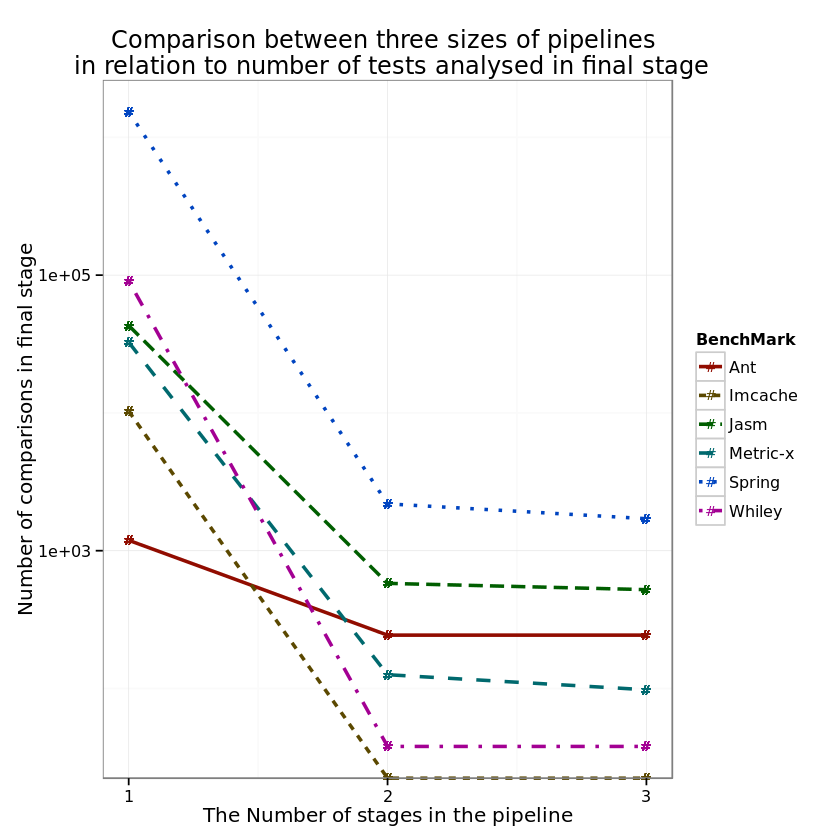
\includegraphics[height=10cm, width = 14.5cm]{Pipeline.png}
\end{center}
\caption{A figure showing the effect that the different pipeline lengths have on the number of comparisons during the final stage (Most computationally heavy). \DIFaddbeginFL \DIFaddFL{It is noted that the number of comparisons for a pipeline of length can be infered from the number of comparisons performed in the first pipeline stage in a pipeline of length two.}\DIFaddendFL }
\label{fig:pipelinegraph}
\end{figure}

\subsection{Discussion}

Inspecting Figure \ref{fig:pipelinegraph}, it becomes clear that the pipeline length \DIFdelbegin \DIFdel{does improve the factors of interest}\DIFdelend \DIFaddbegin \DIFadd{improves the redundant tests in the final stage}\DIFaddend , but the length does not scale in every benchmark. This is shown by every two or three stage pipeline being a significant improvement on a single stage\DIFdelbegin \DIFdel{, however }\DIFdelend \DIFaddbegin \DIFadd{. However }\DIFaddend the majority of the benchmark's perform better with a two stage over a three. These results imply that the \DIFdelbegin \DIFdel{benchmarks that took less time using a two stage, }\DIFdelend \DIFaddbegin \DIFadd{majority of the benchmarks }\DIFaddend were spending more time on the second stage than they were saving from the reduced number of comparisons in the third stage. There \DIFdelbegin \DIFdel{are two scenarios proposed that would cause more time to be spent on the second stage than was saved in the third stage. Firstly, the tool was looking for a different level of similarity between benchmarks, thiswas dependent on how each benchmark reacted to different similarity levels. The benchmarks with unit tests needed to have a higher level of similarity compared to benchmarks with end to end tests. This implies that each benchmark also has its own optimal settings for the second pipeline. The settings were chosen by experimenting with different options, therefore an inefficient second pipeline would have contributed to the result. The second reason }\DIFdelend \DIFaddbegin \DIFadd{is one scenario proposed which would cause this. This scenario }\DIFaddend is that there may be little difference between the outcome from the second and third stages. \DIFdelbegin \DIFdel{An example is shown in }\DIFdelend \DIFaddbegin \DIFadd{Figure \ref{fig:stagesinpipeline} shows that this is what is happening. The figure shows that at the `output' x axis, the majority of benchmarks are under 100 comparisons. This means the next stage would only be performing a small number of comparisons. We would expect that the tests identified at that point are highly redundant. To understand how this affects the outcome, we can inspect }\DIFaddend Figure \ref{fig:pipelinecomp}. Examining the first stage in the pipelines, it shows a large reduction in the number of comparisons. Inspecting the pipeline of length three, the second stage reduces the number of test pairs by a limited amount. This creates a situation where the number of identified redundant test cases has little change from stage two to three while still performing the extra comparisons. \DIFaddbegin \DIFadd{Taking this discussion into account, as well as the factor that a pipeline of length one could take days to complete. }\DIFaddend This leads us to accept the first hypothesis, that increasing the pipeline length \DIFdelbegin \DIFdel{improves the factors of interest, however the optimal length is different for each }\DIFdelend \DIFaddbegin \DIFadd{decreases the time taken and number of comparisons in the final stage. The optimal length of the pipeline may not be the same in every }\DIFaddend benchmark.

The change in the number of redundant tests identified is the other result to examine. The pipeline length of two had no significant difference to a length of three. If there was a change between the pipeline outputs while using the same final stage settings, this could imply two things. Firstly, the second pipeline stage is more specific than the third. Since both pipelines of length two and three share the same settings in final stage, for the pipeline of length three, the second stage may be identifying a higher similarity than the final stage. This would cause a different output between the two lengths. Secondly, there is a bug in the code.

\begin{figure}[h]
\centering
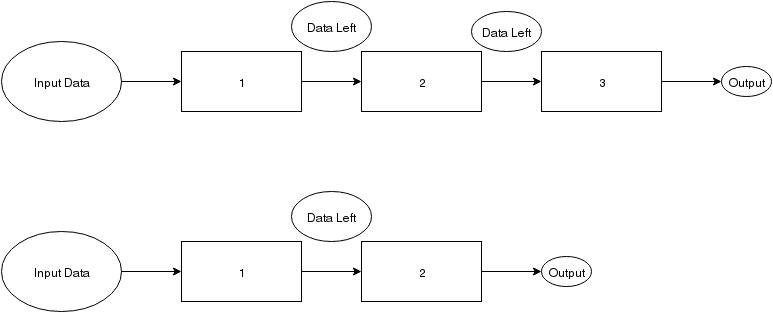
\includegraphics[width=\textwidth,height=8cm]{PipelineComp.png}
\caption{The circle size represents the data that is left in the pipeline. The figure shows that the difference that is between a two stage pipeline and a three stage only has limited room for a reduction in test cases identified. This shows the time taken to execute the extra stage costs more than it saves.}
\label{fig:pipelinecomp}
\end{figure}

\section{Experiment \rom{2} - K Depth Comparison}
\label{kdepthcomp}
\subsection{Motivation}
One of the abilities of the tool is to trace a call tree to the depth of K. This experiment is to determine the impact that altering the depth of K has on the overall cost. 

\begin{hyp}
The precision improvement from increasing K Depth outweighs the performance decrease.
\end{hyp}

Increasing the depth of the call tree leads to an increase in the amount of data that is analysed, intuitively making it more difficult for test cases to be the same. \DIFdelbegin \DIFdel{This should be reflected through }\DIFdelend \DIFaddbegin \DIFadd{We expect }\DIFaddend a reduction in the number of tests identified \DIFaddbegin \DIFadd{to be reflect this }\DIFaddend . The extra data \DIFdelbegin \DIFdel{used causes extra }\DIFdelend \DIFaddbegin \DIFadd{causes more }\DIFaddend analysis, this implies an increase in the time taken as K depth increases. \DIFdelbegin \DIFdel{It is expected }\DIFdelend \DIFaddbegin \DIFadd{We expect }\DIFaddend that the precision increase is worth the performance decrease. \DIFdelbegin \DIFdel{This is reflected in hypothesis 2.
}\DIFdelend \DIFaddbegin \DIFadd{Hypothesis 2 reflects this.
}\DIFaddend 

\subsection{Settings}
There are three K depth's explored, one, two and three respectively. It is important to note that a Wilcoxon signed-rank test was not performed as it is a two-sample test. There were significant tests considered to perform the test for three samples, however we felt the graphs were enough to convey the results.


\subsection{Results}
Ant, Whiley and Spring appear to be the most responsive to the depth of K as shown in Figure \ref{fig:kdepthgraph} albeit by a limited amount. Figure \ref{fig:kdepthtime} shows the differences in time taken. Overall, for every benchmark there wasn't a large amount of change however it shows that as the K depth increases, the time taken increases. \DIFaddbegin \DIFadd{The use of a log scale should be taken into account when looking at the graph. This would make the changes appear less significant. 
}\DIFaddend 

\begin{figure}[h]
\begin{center}
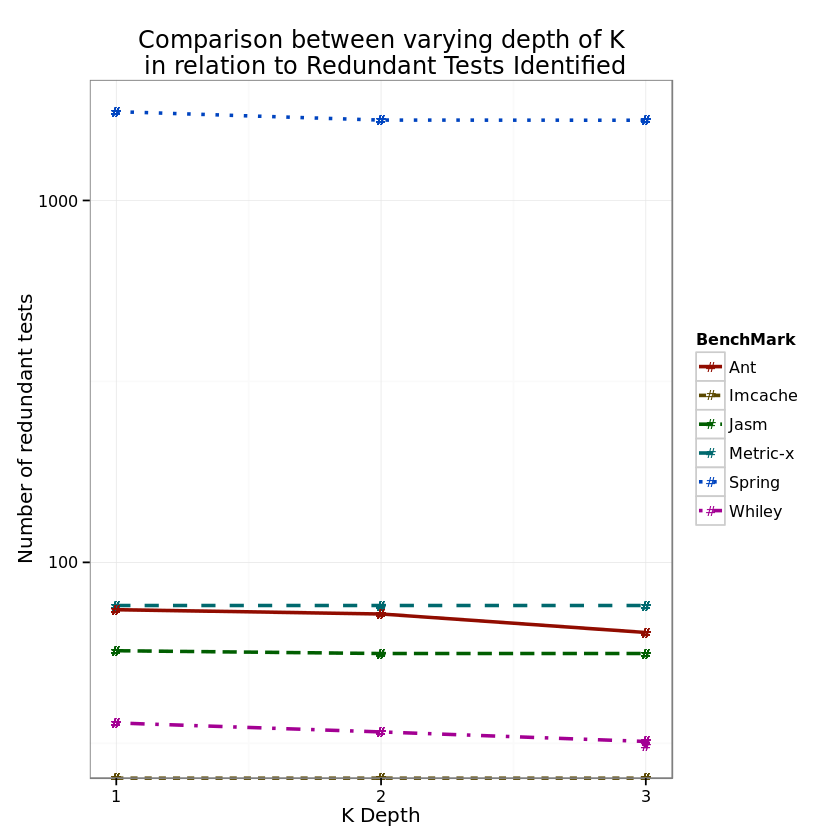
\includegraphics[height=10cm, width = 14.5cm]{KDepth.png}
\end{center}
\caption{A figure showing the effect that a change in the depth of the call tree has on the number of redundant tests are identified.}
\label{fig:kdepthgraph}
\end{figure}

\begin{figure}[h]
\centering
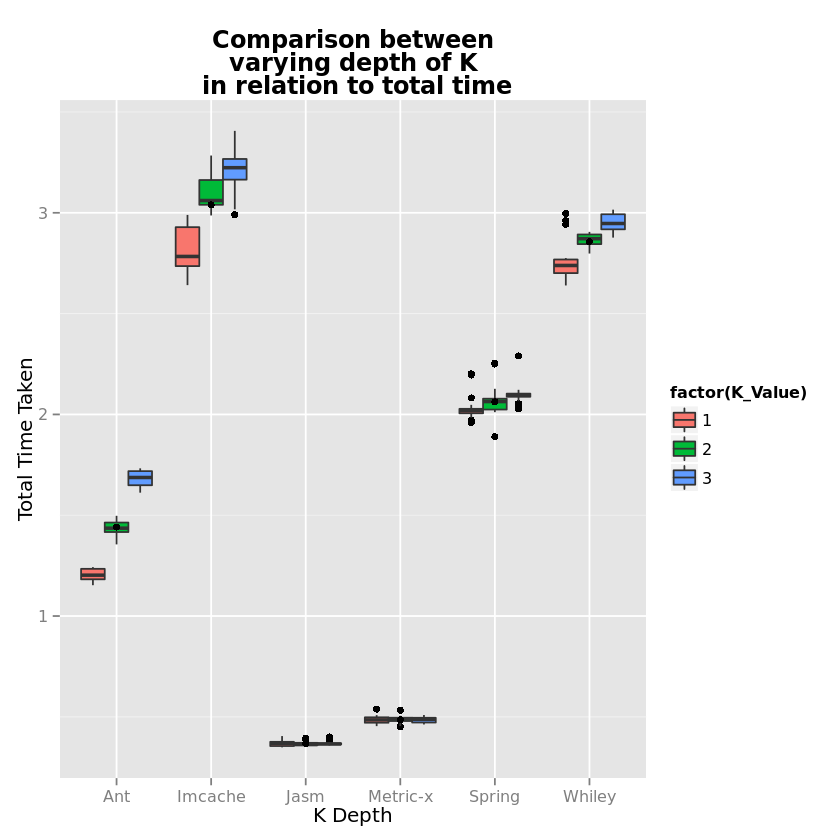
\includegraphics[width=\textwidth,height=13cm]{KDepthTime.png}
\caption{A figure showing the relationship that using a different K Depth has on the total time taken to analyse the data.}
\label{fig:kdepthtime}
\end{figure}

\subsection{Discussion} \DIFaddbegin \improvement{Redo some of this}
\DIFaddend The result shown in Figure \ref{fig:kdepthgraph} shows several things. Firstly, it implies that when no other settings such as weighting or parameters are used, the depth has limited effect on the number of redundant test cases identified. Secondly, the number of comparisons that were output from the first pipeline stage may cause there to be a limited differentiation. When the first pipeline stage outputs a limited number of pairs, the final number of redundant tests identified would be similar regardless of the K depth specified. This situation is similar to the one discussed in Section \ref{sec:pipelineEva} and occurs in Whiley, Metric-x, Imcache and Jasm. The results from this experiment and Experiment \rom{1} indicate that by using a "unique method call" filter and analysing a subset of the data, the tool is able to remove a large majority of the non-redundant tests. \DIFdelbegin \DIFdel{To }\DIFdelend \DIFaddbegin \DIFadd{We can examine Figure \ref{fig:stagesinpipeline} to }\DIFaddend confirm this,  \DIFdelbegin \DIFdel{Figure \ref{fig:stagesinpipeline} can be examined}\DIFdelend . Inspecting the figure, it shows that the heuristic pipeline removes a large portion of the comparisons. It is not enough to confirm the heuristic can reduce comparisons needed, but to inspect the number of tests output. The difference between pipeline stage two and the output is a limited amount. This shows that the heavy computational analysis stage only removes a small set of extra tests, this implies that the heuristic has a good accuracy of identifying redundant tests.
\DIFdelbegin %DIFDELCMD < 

%DIFDELCMD < %%%
\DIFdelend \begin{figure}[h]
\centering
\DIFdelbeginFL %DIFDELCMD < 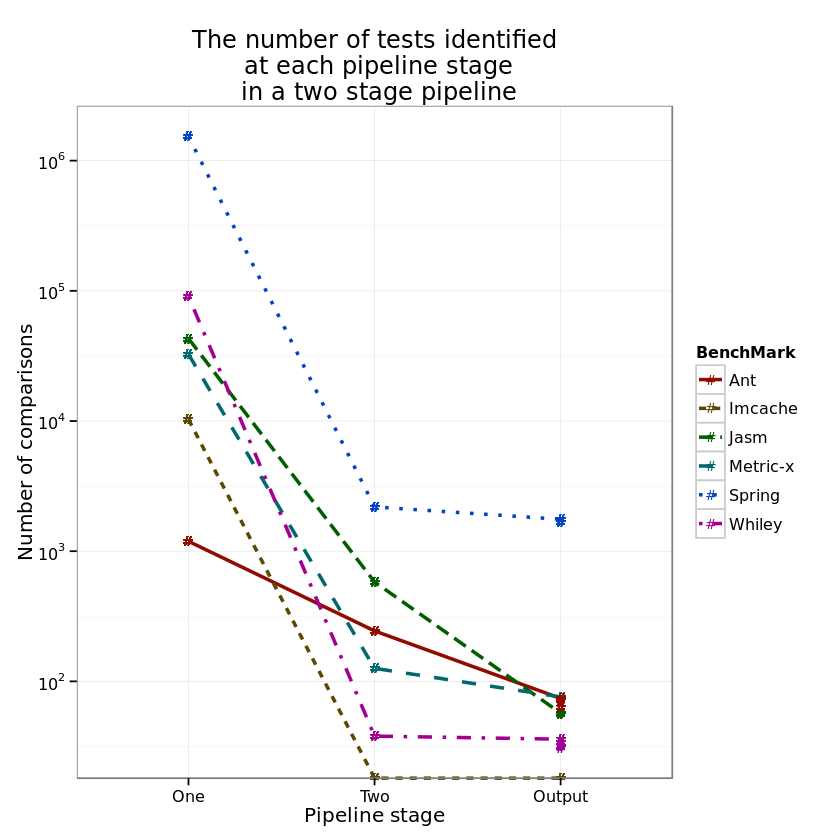
\includegraphics[width=\textwidth,height=13cm]{stagesinpipeline.png}
%DIFDELCMD < %%%
\DIFdelendFL \DIFaddbeginFL 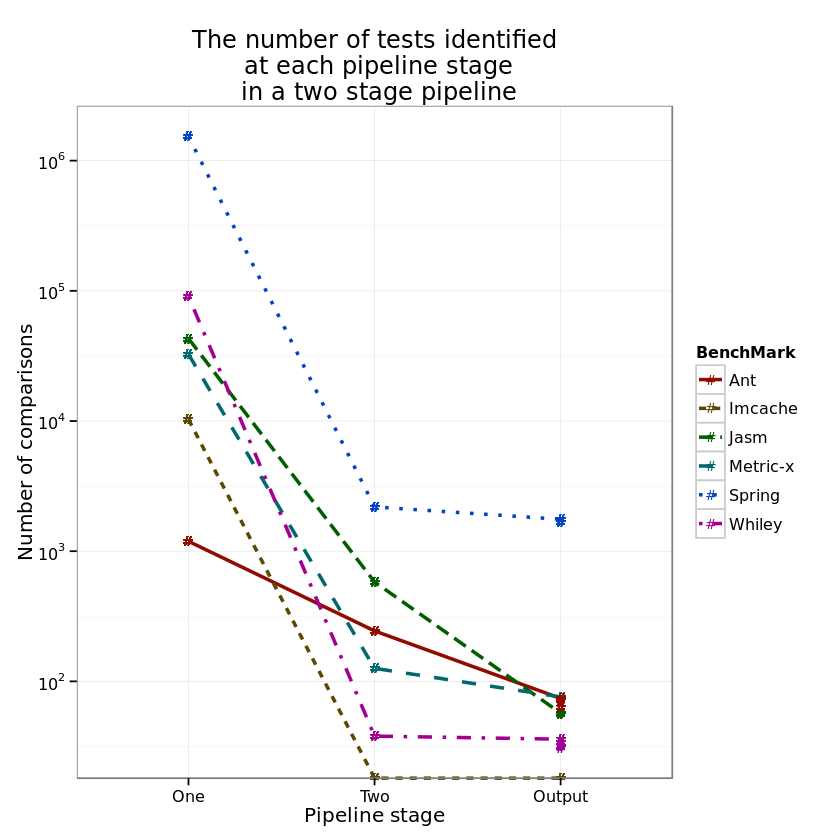
\includegraphics[width=\textwidth,height=11cm]{stagesinpipeline.png}
\DIFaddendFL \caption{A figure showing the the number of comparisons that each stage performs. The pipeline contains two stages and is from Experiment \rom{2}. The graph how the first stage heuristic is able to reduce a large number of the comparisons needed to do for the subsequent stage. \DIFaddbeginFL \textbf{\DIFaddFL{Note}} \DIFaddFL{this differs from Figure \ref{fig:pipelinegraph} as this looks at the number of comparisons in each stage. Figure \ref{fig:pipelinegraph} examines the comparisons performed in the final stage with varying pipeline lengths.}\DIFaddendFL }
\label{fig:stagesinpipeline}
\end{figure}

There is only a limited change in the number of redundant tests identified, however we need to also examine the change in time taken. Increasing the depth of K has varying effect's on the time taken to analyse a benchmarks trace data. \DIFdelbegin \DIFdel{The differences are shown in Figure \ref{fig:kdepthtime} }\DIFdelend \DIFaddbegin \DIFadd{Figure \ref{fig:kdepthtime} shows the differences}\DIFaddend . It shows that Ant, Imcache and Whiley have larger differences than the rest, however in the perspective of time these equate to around half a minute difference. Although increasing the depth has an smaller effect than expected on precision, the impact on time taken isn't substantial. Taking this into account, I can accept the hypothesis with the results implying that for some projects the calling context does not have to be particularly deep. 

\section{Experiment \rom{3} - Parameter Comparison}
\label{sec:param}

\subsection{Motivation}
Parameters show the different contexts that a method was being called in. Retrieving this information gives us more confidence in determining whether two tests are redundant. The experiment explores the impact on performance and precision.

\begin{hyp}
Utilising parameters increases the time taken in comparison to a two stage pipeline.
\end{hyp}

\begin{hyp}
Utilising parameters increases the precision in comparison to a two stage pipeline.
\end{hyp}

\DIFdelbegin \DIFdel{Two factors have to be taken into account }\DIFdelend \DIFaddbegin \DIFadd{We need to take into account two factors }\DIFaddend when discussing the impact of parameters on the time taken. Firstly, it is intuitive that analysing the extra data generated increases the time. The amount of increase is interesting, parameters only add extra computation when the method execution of the given K is exactly the same. For example, if the test execution $A \rightarrow  B \rightarrow  C$ is compared to $A \rightarrow  B \rightarrow  F$ then the parameter won't be taken into account\DIFdelbegin \DIFdel{and therefore }\DIFdelend \DIFaddbegin \DIFadd{. Therefore parameters }\DIFaddend have limited effect on the time taken. 

The amount of time that the VM spends garbage collecting would also increase the time taken\DIFdelbegin \DIFdel{, due to }\DIFdelend \DIFaddbegin \DIFadd{. Due to the }\DIFaddend increased amount of information in memory, the garbage collection process will have to execute more frequently for the analysis to continue to run. This would cause non-deterministic attributes to \DIFdelbegin \DIFdel{be increased. This is reflected in the hypothesises }\DIFdelend \DIFaddbegin \DIFadd{increase. Hypothesis 3 and 4 reflect this. These state }\DIFaddend that parameters increase the precision and the total time taken in comparison to the pipeline of length two in Experiment \rom{1}\DIFaddbegin \DIFadd{.
}\DIFaddend 

\subsection{Settings}
The use of parameters is compared directly to the pipeline of length two used in Experiment \rom{1}.

\subsection{Results}
 \DIFdelbegin \DIFdel{The information for comparing }\DIFdelend \DIFaddbegin \DIFadd{Table \ref{parametersig} shows the comparison information between }\DIFaddend parameters and no parameters\DIFdelbegin \DIFdel{is shown in Table \ref{parametersig}}\DIFdelend . It shows that there was a significant increase for every benchmark in regard to time taken. The table also shows that every benchmark had a significant decrease for the number of redundant test cases identified. This is not the case in Imcache due to it having zero redundant test cases identified in both\DIFdelbegin \DIFdel{, therefore no difference between the two}\DIFdelend . Examining Appendix \ref{fig:paramtime} -- Ant, Imcache, Jasm and Spring appear to affected by an increased variance between executions.

\begin{table}[h]
\centering
\begin{tabular}{|l|l|l|}
\hline
{\bf }          & {\bf Total Time} & {\bf Redundant Tests Identified} \\ \hline
{\bf Whiley}    & +                & -                           \\ \hline
{\bf Jasm}      & +               & -                          \\ \hline
{\bf Ant}       & +                & -                           \\ \hline
{\bf Spring}    & +                & -                           \\ \hline
{\bf Imcache}   & +                & =                           \\ \hline
{\bf Metrics-x} & +                & -                           \\ \hline
\end{tabular}
\caption{A table showing the significant relationship between the use of parameters and no parameters for each benchmark}
\label{parametersig}
\end{table}

\begin{figure}[h]
\begin{center}
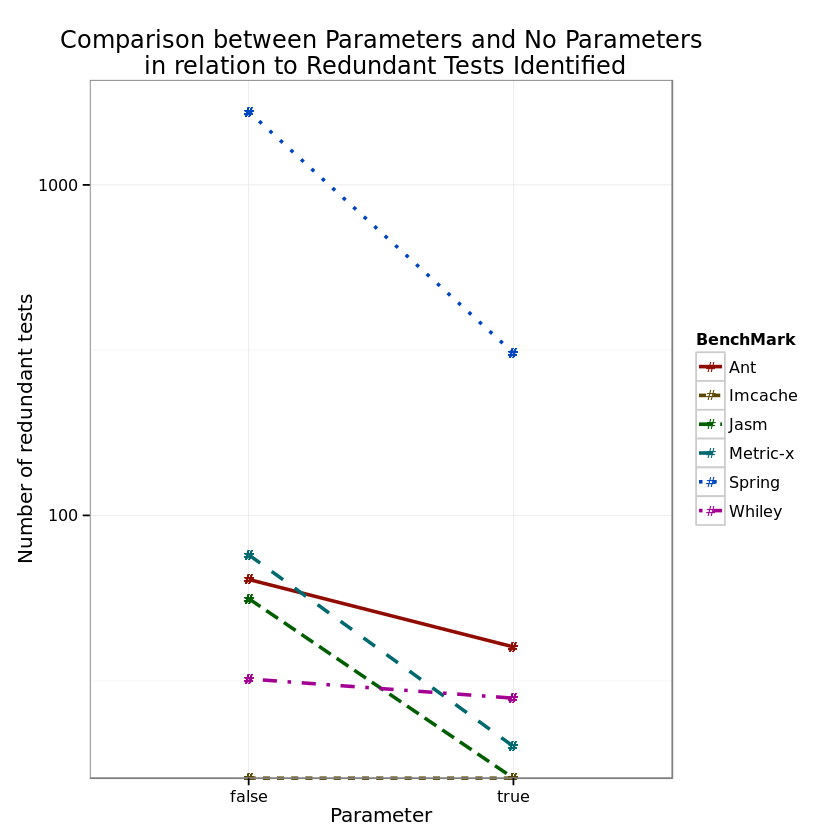
\includegraphics[height=10cm, width = 14.5cm]{Parameters.png}
\end{center}
\caption{A figure showing the effect that using parameters has on the number of redundant tests are identified.}
\label{fig:paramgraph}
\end{figure}


\subsection{Discussion}
The significant Table \ref{fig:paramgraph} matches what is expected. For every benchmark, using parameters significantly increases the time taken. Examining Appendix \ref{fig:paramtime} shows how the benchmarks react with more detail. The most interesting would be Jasm. Without parameters, it analyses the data in less than one minute, with parameters, it takes just under five minutes. This may be indicative of the results discussed in Section \ref{kdepthcomp}. The section discussed how increasing the K depth had little impact on the final outcome. Taking this into account, the call trees were matching the majority of the time and led to parameter information being examined more often, sequentially causing an increase in time taken. A factor that may have an \DIFdelbegin \DIFdel{accumulate effect is related to the setup }\DIFdelend \DIFaddbegin \DIFadd{accumulative effect are the setup and tear down }\DIFaddend methods. If \DIFdelbegin \DIFdel{the set up }\DIFdelend \DIFaddbegin \DIFadd{these }\DIFaddend methods are a large majority of the method calls, and match each other for the K depth, this would further increase the time taken. This allows us to accept hypothesis 3 that parameters increase the time taken.

\DIFdelbegin \DIFdel{Reexamining Table \ref{fig:paramgraph}, it shows that every benchmark had a significant decrease in the number of redundant test cases. }\DIFdelend Looking at Figure \ref{fig:paramgraph}, it confirms that every benchmark reacted with a substantial decrease in redundant tests identified\DIFdelbegin \DIFdel{, with Whiley being }\DIFdelend \DIFaddbegin \DIFadd{. Whiley was }\DIFaddend the least affected. This reiterates the discussion in Section \ref{kdepthcomp} that K depth is not enough of a factor to identify redundant test cases. \DIFdelbegin \DIFdel{It is expected }\DIFdelend \DIFaddbegin \DIFadd{We would expect }\DIFaddend that the number of false positives decrease. Inspecting Table \ref{whileycoding} and \ref{metriccoding} gives insight into the types of tests identified. The Whiley benchmark coding shows that parameters remove the limited redundant tests as well as different array values. The Metric-x coding \DIFdelbegin \DIFdel{demonstrate }\DIFdelend \DIFaddbegin \DIFadd{demonstrates }\DIFaddend a reduction in the number of the different parameter value tests identified substantially, from 52 to 8. Taking these coding tables into account, it allows us to accept hypothesis 4 that parameters increase the precision.

\section{Experiment \rom{4} - Weighting Comparison}
\label{sec:weight}

\subsection{Motivation}
Utilising weighting is an attempt to remove any false positive tests identified. The experiment attempts to identify if applying the weighting technique has potential to remove these false positives\DIFdelbegin \DIFdel{, while exploring }\DIFdelend \DIFaddbegin \DIFadd{. It also provides information concerning }\DIFaddend the impact on performance.

\begin{hyp}
Weighting decreases the number of false positives compared to a standard two stage pipeline
\end{hyp}

\begin{hyp}
Weighting decreases the time taken compared to a standard two stage pipeline
\end{hyp}

As \DIFdelbegin \DIFdel{previously }\DIFdelend discussed in Section \ref{C:related}, much of the related work encountered difficulties with test cases sharing setup and teardown method calls\DIFdelbegin \DIFdel{, resulting }\DIFdelend \DIFaddbegin \DIFadd{. This results }\DIFaddend in a high false positive rate. Intuitively, this makes sense when the test cases are small in comparison to the setup and teardown methods where \DIFdelbegin \DIFdel{the setup and teardown }\DIFdelend \DIFaddbegin \DIFadd{these }\DIFaddend methods represent a large majority of the test data. The approach of removing a \DIFdelbegin \DIFdel{portion }\DIFdelend \DIFaddbegin \DIFadd{part }\DIFaddend of the most executed method calls meant that the amount of data per test case decreases. This should reflect onto the results by showing a decrease in the time taken, as per hypothesis 7. The effect \DIFdelbegin \DIFdel{that it }\DIFdelend \DIFaddbegin \DIFadd{the weighting technique }\DIFaddend has on the number of redundant test cases should be dependent on the benchmark\DIFdelbegin \DIFdel{when weighting is used}\DIFdelend . This is because removing the most common tests should imply a decreased false-positive rate, but also may increase the number of actual redundant tests picked up. \DIFdelbegin \DIFdel{The precision is of interest when examining the cause effect of weighting, this is reflected by hypothesis 6.
}\DIFdelend \DIFaddbegin \DIFadd{Hypothesis 6 reflects  our interest in the precision difference.
}\DIFaddend 

\subsection{Settings}
The use of weighting is compared directly to the pipeline of length two settings in Experiment \rom{1}.


\subsection{Results}
There are a mixture of results \DIFdelbegin \DIFdel{in regard to }\DIFdelend \DIFaddbegin \DIFadd{concerning }\DIFaddend the total time taken. We see this in Table \ref{weightingsig} -- Whiley, Ant and Imcache had a significant increase in the time taken to analyse. Jasm, Spring and Metric-x had a significant decrease in the time taken to analyse. The majority -- Whiley, Ant, Jasm and Metrics-x had a significant decrease in the number of redundant tests identified. Spring was the only benchmark where weighting significantly \DIFdelbegin \DIFdel{increase }\DIFdelend \DIFaddbegin \DIFadd{increased }\DIFaddend the number of redundant tests identified.

\begin{table}[h]
\centering


\begin{tabular}{|l|l|l|}
\hline
{\bf }          & {\bf Total Time} & {\bf Redundant Tests Identified} \\ \hline
{\bf Whiley}    & +                & -                           \\ \hline
{\bf Jasm}      & -                & -                           \\ \hline
{\bf Ant}       & +                & -                           \\ \hline
{\bf Spring}    & -                & +                           \\ \hline
{\bf Imcache}   & +                & =                           \\ \hline
{\bf Metrics-x} & -                & -                           \\ \hline
\end{tabular}
\caption{A table showing the significant relationship between the use of weighting and no weighting for each benchmark}
\label{weightingsig}
\end{table}


\begin{figure}[h]
\begin{center}
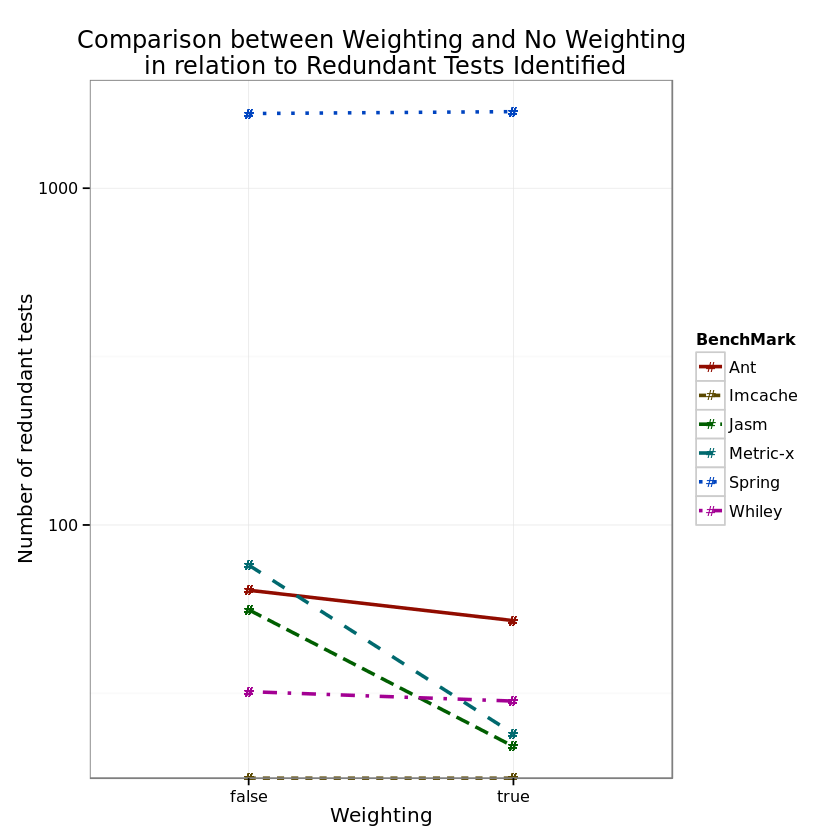
\includegraphics[height=10cm, width = 14.5cm]{Weighting.png}
\end{center}
\caption{A figure showing the effect that using weighting has on the number of redundant tests are identified.}
\label{fig:weightgraph}
\end{figure}

\subsection{Discussion}
A reduction in the false positive rate was \DIFdelbegin \DIFdel{weighting's }\DIFdelend \DIFaddbegin \DIFadd{the weighting techniques }\DIFaddend primary goal. Spring was the only benchmark that had a significant increase in the number of redundant test cases identified. The other benchmarks had a significant decrease. At first, this makes it appear that by using weighting it may solve some of the issues \DIFdelbegin \DIFdel{that were identified in \mbox{%DIFAUXCMD
\cite{koochakzadeh2009test}
}%DIFAUXCMD
\mbox{%DIFAUXCMD
\cite{li2008static}
}%DIFAUXCMD
}\DIFdelend \DIFaddbegin \DIFadd{Maurer et al  \mbox{%DIFAUXCMD
\cite{koochakzadeh2009test}
}%DIFAUXCMD
and Robinson et al. \mbox{%DIFAUXCMD
\cite{li2008static}
}%DIFAUXCMD
identified}\DIFaddend . To confirm this, examining Table \ref{whileycoding} and \ref{metriccoding} will give insight into the effect of weighting. Comparing the two columns for the Whiley coding, Pipeline 2 and Weighting, the only difference is the removal of the two limited redundancy test cases that were picked up by Pipeline 2. This shows the weighting technique is able to reduce the impact that the similar set up and tear down methods have on the analysis. By removing the method executions that were common, this led to a decrease in the number of false positive tests identified. The Metric-x coding is a similar result. The weighting technique reduces the number of parameter value redundancies identified as well as the limited redundancies, \DIFdelbegin \DIFdel{however }\DIFdelend \DIFaddbegin \DIFadd{but }\DIFaddend does not completely remove them. This is interesting and implies that the number of setup and tear down methods that remained in the data analysed was still a large \DIFdelbegin \DIFdel{portion }\DIFdelend \DIFaddbegin \DIFadd{part }\DIFaddend of the data. We are able to accept hypothesis 6, although work remains to improve the weighting method to remove redundant tests completely.

Table \ref{weightingsig} shows a mixture of results in regard to the total time taken. Two out of the three benchmarks that had a significant increase in the total time were small benchmarks -- Whiley, Ant, Imcache. This may imply that the size of the benchmark has some relation to the effect of weighting on the time taken. One reason is that \DIFdelbegin \DIFdel{weighting is calculated }\DIFdelend \DIFaddbegin \DIFadd{the tool calculates weighting }\DIFaddend once per test case per analysis stage. The weighting calculation has a linear relation with the number of test cases. In comparison, \DIFaddbegin \DIFadd{the tool compares }\DIFaddend every test case \DIFdelbegin \DIFdel{is compared }\DIFdelend to every other\DIFdelbegin \DIFdel{, therefore a n-squared }\DIFdelend \DIFaddbegin \DIFadd{. This is a squared }\DIFaddend relation with the number of test cases. The less test cases there are, the closer the linear relation is to the \DIFdelbegin \DIFdel{n }\DIFdelend squared and the more impact the linear weight calculation has on the \DIFdelbegin \DIFdel{overall }\DIFdelend time taken. This may explain a relation between size and time taken. \DIFdelbegin \DIFdel{The the overall }\DIFdelend \DIFaddbegin \DIFadd{Appendix \ref{fig:weighttime} shows the overview of the }\DIFaddend impact on the time taken \DIFdelbegin \DIFdel{is shown in Appendix \ref{fig:weighttime}}\DIFdelend . The figure shows there was no general impact from using weighting on the benchmarks. Taking the discussion into account, it allows us to invalidate hypothesis \DIFdelbegin \DIFdel{7.
}\DIFdelend \DIFaddbegin \DIFadd{7 and that weighting does not affect time taken.
}\DIFaddend 

\section{Redundant Test Case Coding}

\DIFdelbegin %DIFDELCMD < \improvement{I think discuss some here}
%DIFDELCMD < %%%
\DIFdelend \DIFaddbegin \DIFadd{Tables \ref{whileycoding} and \ref{metriccoding} are the tests identified coded under a type of redundancy. These types of redundancies allow us to see how many false-positives occured. These coding have been referred to in Section \ref{sec:param} and Section \ref{sec:weight}. However neither weighting or parameters were able to fully remove the tests with limited redundancy in Table \ref{metriccoding}. The table suggests that the combination of parameters and weighting may have some appeal by removing all eight limited redundancy tests. At the same time, the similar tests are also removed which is a negative outcome. This suggests that the combination may have some applicability to other benchmarks and may warrant future experiments on it.
}\DIFaddend 

\begin{table}[h]
\centering

\begin{tabular}{|l|l|l|l|l|}
\hline
                          & \multicolumn{4}{c|}{{\bf Whiley}}                                                             \\ \hline
{\bf Types of redundancy} & \multicolumn{1}{c|}{{\bf Pipeline 2}} & {\bf Weighting} & {\bf Parameters} & {\bf Parameters and Weighting} \\ \hline
Different Equation Value  & 6                                     & 6               & 6                & 6                \\ \hline
Different Equation Sign   & 8                                     & 8               & 8                & 8                \\ \hline
Different Array Values    & 2                                     & 2               & 0                & 0                \\ \hline
Same                      & 10                                    & 10              & 10               & 10               \\ \hline
Limited Redundancy        & 2                                     & 0               & 0                & 0                \\ \hline
Rearranged Equation       & 2                                     & 2               & 2                & 2                \\ \hline
Extra if statement        & 2                                     & 2               & 2                & 2                \\ \hline
                          &                                       &                 &                  &                  \\ \hline
{\bf Total}               & 32                                    & 30              & 28               & 28               \\ \hline
\end{tabular}
\caption{A table displaying a list of coding's for the Whiley Benchmark for four of the different techniques used. \DIFaddbeginFL \DIFaddFL{The tests identified have been coded under a type of redundancy. These types of redundancies allow us to see how many false-positives were identified as being redundant. }\DIFaddendFL }
\label{whileycoding}
\end{table}


\begin{table}[]
\centering
\begin{tabular}{|l|l|l|l|l|}
\hline
                             & \multicolumn{4}{c|}{\textbf{Metric-X}}                                                              \\ \hline
\textbf{Types of redundancy} & \textbf{Pipeline 2} & \textbf{Weighting} & \textbf{Parameters} & \textbf{Parameters  And Weighting} \\ \hline
Different Parameter Value    & 52                  & 10                 & 8                   & 4                                  \\ \hline
Different Object Type        & 6                   & 2                  & 2                   & 0                                  \\ \hline
Different Array Values       & 8                   & 6                  & 4                   & 6                                  \\ \hline
Similar                      & 2                   & 2                  & 0                   & 0                                  \\ \hline
Limited Redundancy           & 8                   & 4                  & 6                   & 0                                  \\ \hline
\textbf{}                    &                     &                    &                     &                                    \\ \hline
\textbf{Total}               & 76                  & 24                 & 20                  & 10                                 \\ \hline
\end{tabular}
\caption{A table displaying a list of coding's for the Whiley Benchmark for four of the different techniques used. \DIFaddbeginFL \DIFaddFL{The tests identified have been coded under a type of redundancy. These types of redundancies allow us to see how many false-positives were identified as being redundant.}\DIFaddendFL }
\label{metriccoding}
\end{table}

\section{Limitations\DIFdelbegin %DIFDELCMD < \improvement{Dave}%%%
\DIFdelend }

\DIFaddbegin \begin{itemize}

\item \DIFaddend A major limitation to the study was \DIFdelbegin \DIFdel{volatile memory}\DIFdelend \DIFaddbegin \DIFadd{the amount of RAM used}\DIFaddend . For the \DIFdelbegin \DIFdel{test suites }\DIFdelend Whiley and Ant \DIFdelbegin \DIFdel{, }\DIFdelend \DIFaddbegin \DIFadd{benchmarks, the tool had high RAM usage when }\DIFaddend storing the parameter data and call tree \DIFdelbegin \DIFdel{endured a high level of volatile memory usage, limiting }\DIFdelend \DIFaddbegin \DIFadd{information. This limited }\DIFaddend the amount of tests that \DIFdelbegin \DIFdel{were able to be retrieved. An approach that should have been considered with more thought was the use of a database.
Although this would have introduced difficulty reducing the non-deterministic behaviour to a minimum. A major factor would be the difficulty around executing the analysis on a grid system and replicating the conditions each run.
}\DIFdelend \DIFaddbegin \DIFadd{it was able to retrieve. The experiments may not fully represent the total redundancy in these two benchmarks.
}\DIFaddend 

\DIFaddbegin \item \DIFaddend Some of the benchmarks that \DIFdelbegin \DIFdel{were chosen }\DIFdelend \DIFaddbegin \DIFadd{we chose }\DIFaddend contain multiple unit tests within one test case. The tool described throughout this \DIFdelbegin \DIFdel{paper }\DIFdelend \DIFaddbegin \DIFadd{report }\DIFaddend would not be able to pick up when a test case subsumes another. The \DIFdelbegin \DIFdel{frame work }\DIFdelend \DIFaddbegin \DIFadd{tool }\DIFaddend only looks at the \DIFdelbegin \DIFdel{total method set, and for each of the singular unit tests, there would need to be a skewed proportion of the conjoined test case in regard to the total method executions. This means that unless one of the unit tests within the conjoined test case was arbitrary larger than the other then it would not be picked up as being redundant, unless there was another conjoined test case similar.
This is where the other approaches identified in the related work would be more effective. By looking at the statement information, it is easier to determine when a test is a subset of another.
}\DIFdelend \DIFaddbegin \DIFadd{method call information, as such gains no new information by identifying method call subsumed tests. It is then difficult gauge this type of redundancy within the test suites.
}\DIFaddend 

\DIFdelbegin \DIFdel{As discussed in Section \ref{sec:pipelineEva}, some }\DIFdelend \DIFaddbegin \item \DIFadd{Some }\DIFaddend benchmarks performed better with a two stage pipeline in comparison to a three stage, and vice versa. \DIFdelbegin \DIFdel{This may have been due to not being able to identify the optimal parameters for each benchmark, although there were multiple different parameters tested to explore each benchmark's optimal . }%DIFDELCMD < \todo{Maybe explore how I decided the optimal ?}
%DIFDELCMD < %%%
\DIFdelend \DIFaddbegin \DIFadd{A range of different settings were tested to identify close to optimal settings for the second stage. However, this does not mean that the settings chosen were optimal and may have skewed the data slightly.
}\DIFaddend 

\DIFdelbegin %DIFDELCMD < \todonote{Discussed how weighting is applied each stage, but this would be computing redundant information. However, this does not affect the experiments as weighting is ever only executed once per pipeline.}
%DIFDELCMD < 

%DIFDELCMD < %%%
\section{%DIFDELCMD < \improvement{Summary?}%%%
\DIFdel{Summary}}
%DIFAUXCMD
\addtocounter{section}{-1}%DIFAUXCMD
%DIFDELCMD < 

%DIFDELCMD < \todonote{summarise the experiments} %%%
\DIFdelend \DIFaddbegin \item \DIFadd{The tool applies the weighting technique once per stage where required. Performing the calculation once per stage is adds unnecessary calculations. This does not affect the experiments as weighting is ever only executed once per pipeline.
}\end{itemize}
 \DIFaddend \newpage 
 \newpage \chapter{Future Work and Conclusions\DIFdelbegin %DIFDELCMD < \improvement{Dave}%%%
\DIFdelend }\label{C:future}

This chapter will first discuss potential future work which would increase the usefulness of the tool for a wider range of audiences. The experiments are then reflected on and finally concluded. 
\DIFdelbegin %DIFDELCMD < \todo{Finish properly}
%DIFDELCMD < %%%
\DIFdelend 

\section{Future Work}
\DIFdelbegin \DIFdel{The tool created throughout the project allows for the trace information from a test suite to be stored and analysed using different techniques. The information we explored using to determine redundant tests was the method calls. }\DIFdelend Throughout the project, three main areas have been identified for future work\DIFaddbegin \DIFadd{: The ability to handle larger test suites, tracing statement information and lastly, using both statement and method information together}\DIFaddend .

\begin{itemize}

\item \textbf{Handle larger test suites.} The main objective would be to increase the ability of the tool to handle larger test suites. Currently, the tool relies on RAM to hold the trace and analysis information however, the amount of data held can often grow rapidly if the test cases contain a large number of method calls. An approach to get around this would be to integrate the tool with a database. \DIFaddbegin \todonote{This was achieved in Nelsons.....} \DIFaddend This would allow the tool to handle arbitrary large suites. The down side would \DIFaddbegin \DIFadd{that }\DIFaddend the speed of the tool would decrease as the read/write to disk is slower than to RAM. \DIFaddbegin \DIFadd{This may be negligible as databases optimize their read and write by using a certain amount of memory. }\DIFaddend Giving developers this option would \DIFdelbegin \DIFdel{be preferred}\DIFdelend \DIFaddbegin \DIFadd{increases the capability of the tool}\DIFaddend . 

\item \textbf{Trace statement information.} The tool has the ability to trace method call information and has potential to be used on large test suites. This approach may not be the best when we are only looking at smaller test suites. Another approach that could be implemented is tracing the statement coverage information. This would allow us to compare the statement and method coverage information directly and give us more insight into the issue of identifying redundant tests. Tracing the statement information would allow us to further explore the use case mentioned in Chapter \ref{C:intro}. The use case was the ability to split the test suites into two, one containing the non redundant test cases and the other was the original suite. This could be further expanded with statement coverage information. By identifying when a test subsumes another, the test subsumed could be moved into another suite. If the larger test fails, the subsumed tests could then be ran to help pin point the error in the code.

\item \textbf{Combining Statement and method information.} The method call information was a good heuristic to use. On the other hand, it is difficult to judge how good method calls are \DIFdelbegin \DIFdel{overall }\DIFdelend at identifying redundant test cases without any comparison to statement coverage or \DIFdelbegin \DIFdel{purposeful }\DIFdelend \DIFaddbegin \DIFadd{large scale }\DIFaddend redundancy and bugs added. One application could be to combine the statement and method information together. \DIFdelbegin \DIFdel{Method information could be used }\DIFdelend \DIFaddbegin \DIFadd{The tool could use the method information }\DIFaddend as a heuristic and statement coverage could then explore the test cases identified by the heuristic.

\end{itemize}

\section{Conclusions}

There were two main contributions of the paper as discussed in Chapter \ref{C:intro}:

\begin{itemize}
\item Create a tool for identifying redundant test cases (Chapter 3)
\item Analyse different strategies for identifying redundant test cases through experimenting on realistic benchmarks (Chapter 4)
\end{itemize}

Throughout the report, the tool has been discussed along with the different techniques implemented. The tool first had to trace the data. This was achieved through the \DIFdelbegin \DIFdel{Aspectj }\DIFdelend \DIFaddbegin \DIFadd{AspectJ }\DIFaddend framework. After the test suites were able to be traced, the trace information then had to be filtered with different spectra. The ability to filter out information was one of the key features of the tool. This allowed developers to trace information, then run a range of different filters over the data without being constrained to one spectra. The three spectra filters were ``unique method calls", ``all method calls" and "call tree". The other key feature of the tool was the pipeline. Integrating it with the spectra filters allowed for the "unique method calls" to be used as a heuristic to reduce the number of comparisons that the subsequent stages had to perform. The tool then was altered to trace the parameter information from the test cases. This was achieved by using reflection on the parameter objects. Finally, the ability to apply a weighting was implemented. This was achieved by removing the top 20\% method calls.

\paragraph{Method Call Information}
The use of method call information was a good candidate to identify redundant tests. They allow the tool to look at test suites that produce a larger amount of total information, in particular ones which are end to end tests -- Whiley and Jasm. As mentioned in the Future Work section above and discussed in Experiment \rom{2}, the method calls appeared to be particularly good at being \DIFaddbegin \DIFadd{used as }\DIFaddend a heuristic. Filtering with the "unique method calls" spectra, the tool was able to remove a large portion of the test case comparisons in the final stage had to perform \DIFaddbegin \DIFadd{while retaining good precision}\DIFaddend .

\paragraph{Pipeline}
Pipelining was one of the critical aspects of the project. It not only lead to a decrease in the time taken but also the memory consumed. An important thing to note is each benchmark had an optimal length of the pipeline, using a length larger \DIFaddbegin \DIFadd{than the optimal }\DIFaddend caused more time to be taken to analyse than was saved. Pipelining particularly worked well with the use of a \DIFdelbegin \DIFdel{heuristic }\DIFdelend \DIFaddbegin \DIFadd{"unique method call" spectra }\DIFaddend filter.

\paragraph{Call tree depth}
The experiments showed that as the depth of the call tree increased, there was limited level of reduction in the number of redundant tests identified. This result was unexpected. Although there was a change, it was lower that what was expected. This implies that by increasing the K depth without any other technique, there is limited improvement. 

\paragraph{Parameter}
By using reflection to retrieve the fields of these objects it allowed more insight into the content that the parameter objects were holding and the nature of them, but it also meant more data had to be held and analysed resulting in an increased time taken. There exists this trade off between time taken and confidence of redundancy when using parameters. 

\paragraph{Weighting}
The weighting technique implemented attempts to improve the accuracy of the tool by removing false-positives while improving the time taken to analyse. Experiment \rom{4} discussed how weighting was able to reduce the level of false-positives but needs further improvement.

\DIFdelbegin \subsection{\DIFdel{Conclusion}}
%DIFAUXCMD
\addtocounter{subsection}{-1}%DIFAUXCMD
%DIFDELCMD < 

%DIFDELCMD < %%%
\DIFdelend \DIFaddbegin \paragraph{}
\DIFaddend The project has explored the use of higher level information than previously explored for identifying redundant test cases while examining how different techniques can impact the results. The output of the tool is adequate in the sense that there is a low number of tests identified and these tests contain limited non-redundant tests\DIFdelbegin \DIFdel{. 
}%DIFDELCMD < 

%DIFDELCMD < %%%
\DIFdel{The results would be expected to build off those achieved in Maurer et al. \mbox{%DIFAUXCMD
\cite{li2008static}
}%DIFAUXCMD
and Robinson et al. \mbox{%DIFAUXCMD
\cite{koochakzadeh2009test}
}%DIFAUXCMD
}\DIFdelend . 


 \newpage 
 \newpage \begin{appendices}
\chapter{The effect of pipeline size in regard to the time taken}
\begin{figure}[h]
\centering
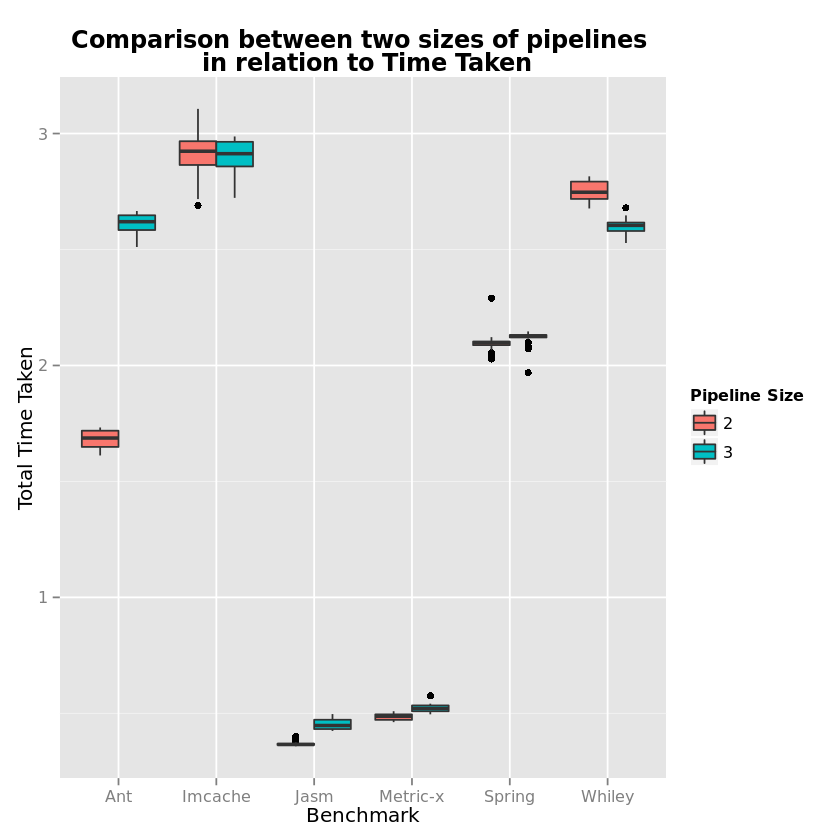
\includegraphics[width=\textwidth,height=13cm]{PipelineTime.png}
\caption{A figure showing the relationship that using different pipeline sizes has on the total time taken to analyse the data.}
\label{fig:pipelinetime}
\end{figure}

\chapter{The effect of parameters in regard to the time taken}
\begin{figure}[h]
\centering
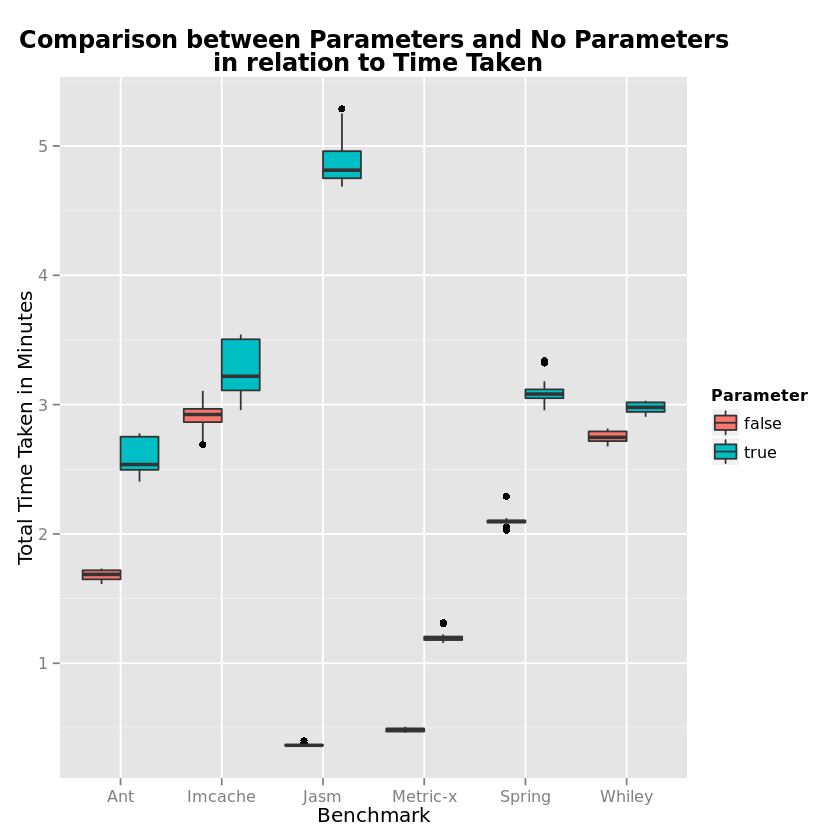
\includegraphics[width=\textwidth,height=13cm]{ParamTime.png}
\caption{A figure showing the relationship that using parameters has on the total time taken to analyse the data.}
\label{fig:paramtime}
\end{figure}

\chapter{The effect of weighting in regard to the time taken}
\begin{figure}[h]
\centering
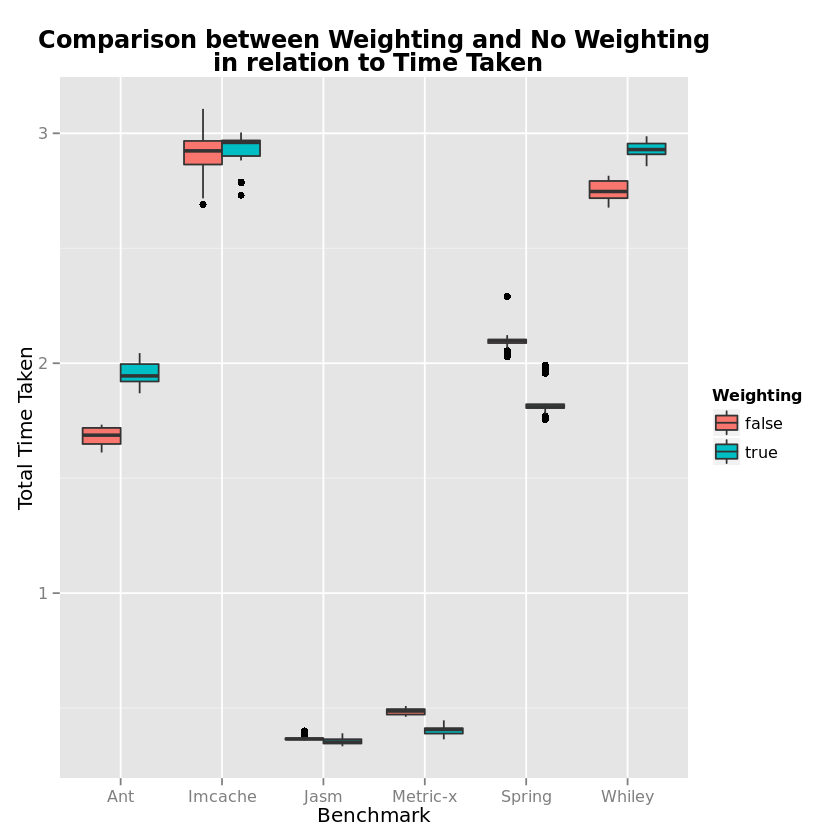
\includegraphics[width=\textwidth,height=13cm]{WeightTime.png}
\caption{A figure showing the relationship that using weighting has on the total time taken to analyse the data.}
\label{fig:weighttime}
\end{figure}

\chapter{The effect of weighting and parameters combined in regard to the time taken}
\begin{figure}[h]
\centering
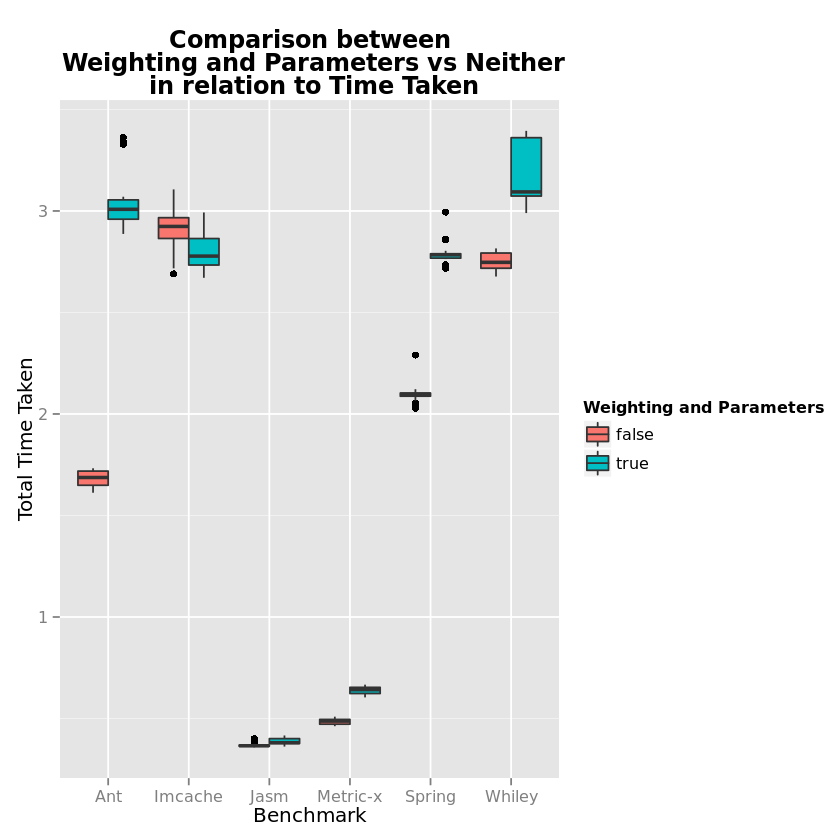
\includegraphics[width=\textwidth,height=13cm]{WeightnParamTime.png}
\caption{A figure showing the relationship that using weighting and parameters combined has on the total time taken to analyse the data.}
\label{fig:weightparamtime}
\end{figure}

\chapter{The effect of weighting and parameters vs parameters in regard to the time taken}
\begin{figure}[h]
\centering
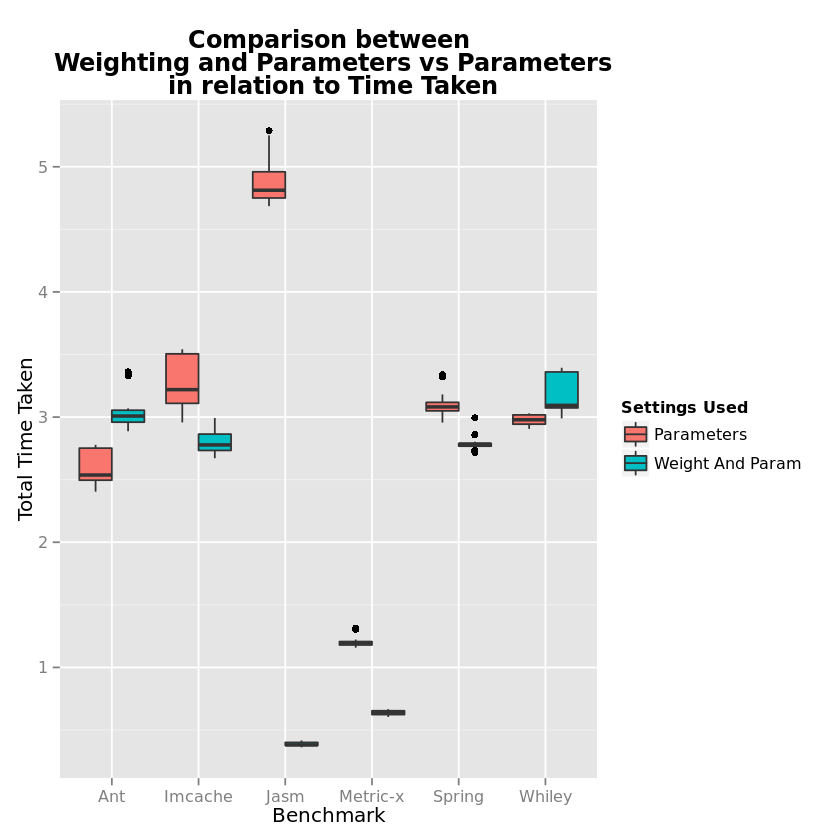
\includegraphics[width=\textwidth,height=13cm]{WeightnParamvParamTime.png}
\caption{A figure showing the relationship that using weighting and parameters combined vs parameters alone has on the total time taken to analyse the data.}
\label{fig:weightparamvparamtime}
\end{figure}




\end{appendices} \newpage 

%%%%%%%%%%%%%%%%%%%%%%%%%%%%%%%%%%%%%%%%%%%%%%%%%%%%%%%

\backmatter

%%%%%%%%%%%%%%%%%%%%%%%%%%%%%%%%%%%%%%%%%%%%%%%%%%%%%%%


%\bibliographystyle{ieeetr}
\bibliographystyle{acm}
\bibliography{sample.bib}


\end{document}
